\documentclass[12pt,a4paper,landscape]{article}
\usepackage[utf8]{inputenc}
\usepackage[T1]{fontenc}
\usepackage{graphicx}
\usepackage{booktabs}
\usepackage[margin=0.5in, top=0.5in, headsep=0.1in]{geometry}
\usepackage{caption}
\usepackage{float}
\usepackage[authoryear,round]{natbib}
\usepackage{xcolor}
\usepackage{colortbl}
\usepackage{rotating}
\usepackage{tabularx}
\usepackage{pdflscape}
\usepackage{adjustbox}
\usepackage{times}
\usepackage{array}
\usepackage{fancyhdr}
\usepackage[colorlinks=true, allcolors=blue]{hyperref}

% Setup fancy headers
\fancypagestyle{mainStyle}{%
    \fancyhf{}
    \renewcommand{\headrulewidth}{0pt}
    \fancyhead[R]{\footnotesize\hyperref[toc]{Back to Contents}}
}

\pagestyle{mainStyle}

\newcommand{\countryheader}[2]{\large\bfseries\hyperref[#1]{#2}}
\captionsetup[table]{labelformat=empty}
\definecolor{lightgray}{gray}{0.85}

\begin{document}
\title{\Large Country Data and Graphs for Uzbekistan}
\date{June 30, 2025}
\maketitle
\thispagestyle{empty}

\clearpage
\setcounter{page}{1}
\hypersetup{colorlinks=true,linkcolor=blue,linktoc=all}
\phantomsection
\label{toc}
\tableofcontents
\thispagestyle{empty}
\clearpage
\phantomsection
\addcontentsline{toc}{section}{Data availability heatmap}
\begin{center}
{\Large\bfseries Data availability heatmap}
\end{center}
\vspace{1cm}
\begin{figure}[H]
\centering
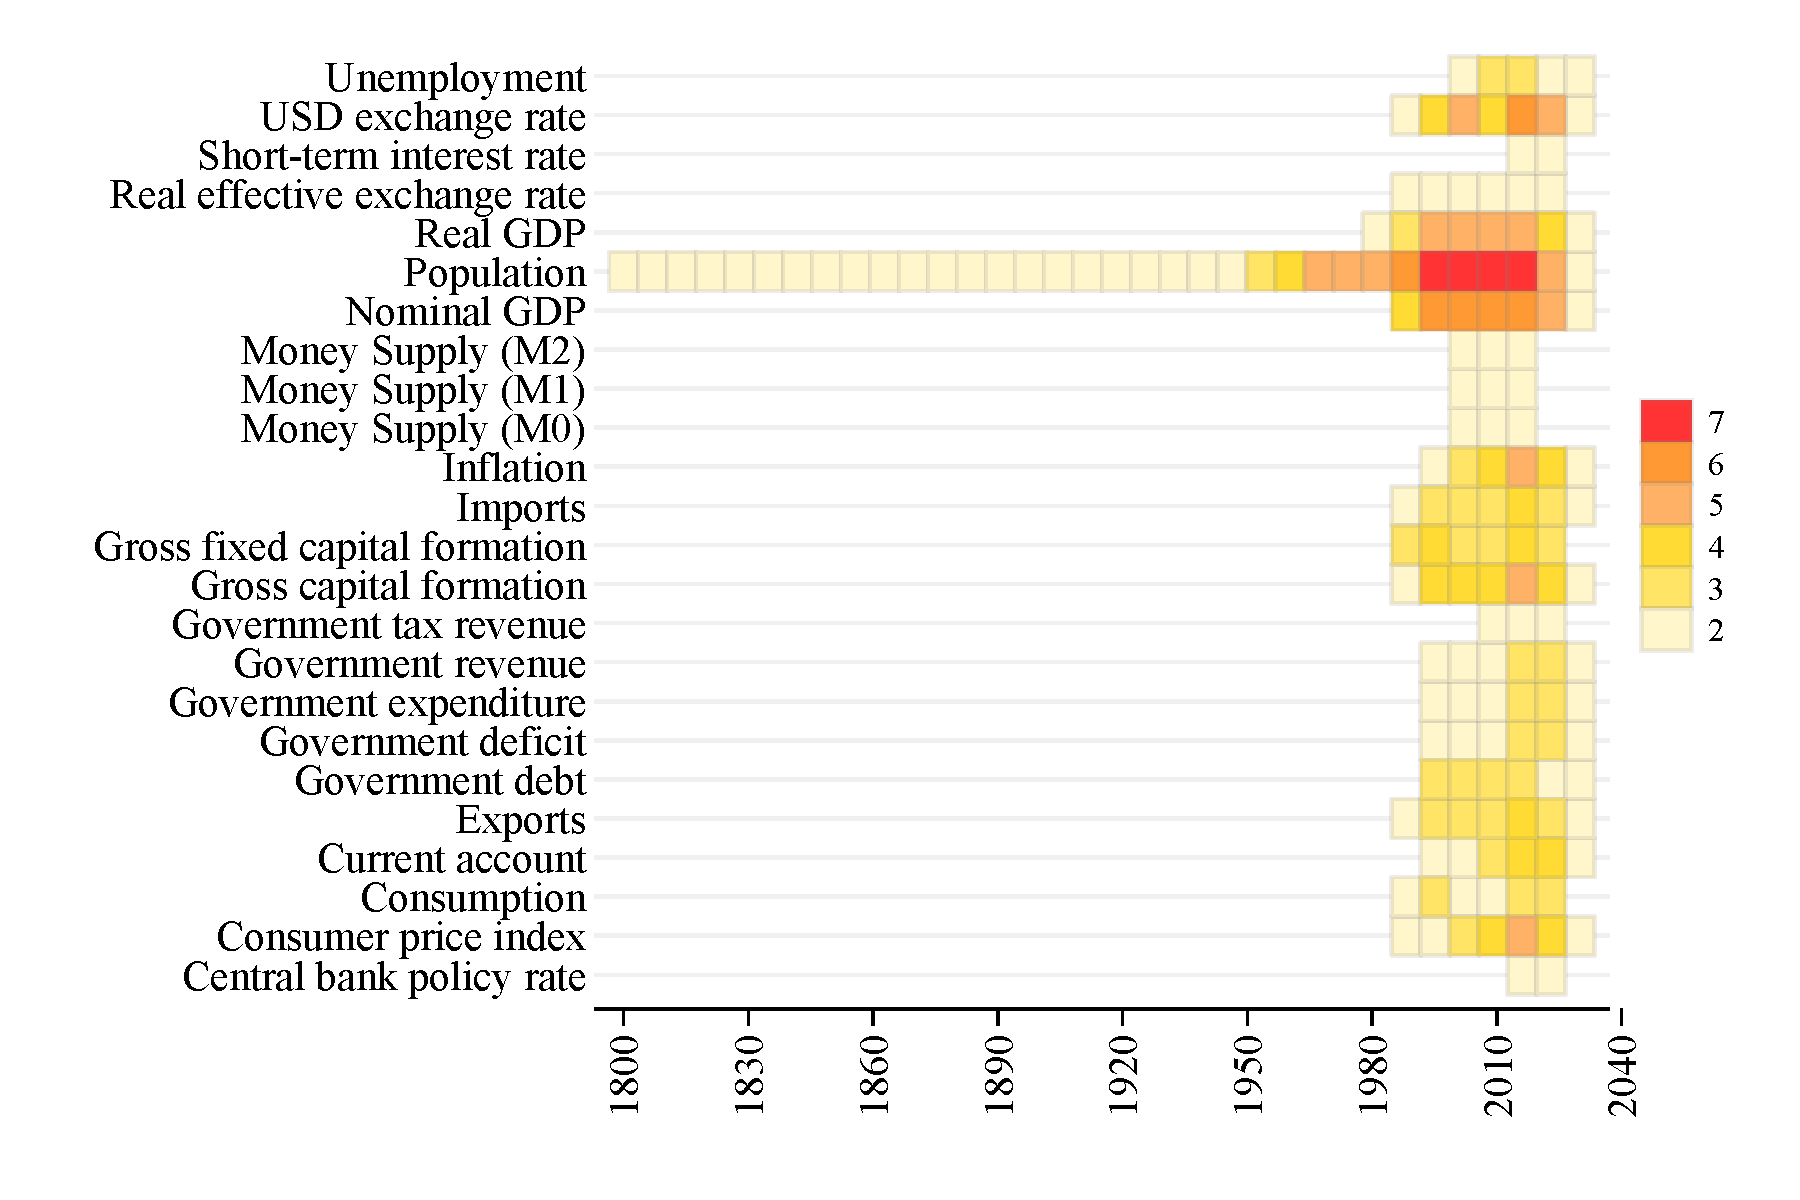
\includegraphics[width=\textwidth,height=0.8\textheight,keepaspectratio]{graphs/UZB_heatmap.pdf}
\end{figure}
\setcounter{page}{3}
\begin{adjustbox}{max totalsize={\paperwidth}{\paperheight},center}
\begin{minipage}[t][\textheight][t]{\textwidth}
\vspace*{0.5cm}
\phantomsection
\addcontentsline{toc}{section}{Current account balance}
\begin{center}
{\Large\bfseries Current account balance}
\end{center}
\vspace{0.5cm}
\begin{table}[H]
\centering
\small
\begin{tabular}{|l|l|l|}
\hline
\textbf{Source} & \textbf{Time span} & \textbf{Notes} \\
\hline
\rowcolor{white}\cite{WDI_ARC}& 1992 - 1997 &Spliced using overlapping data in 1998. \\
\rowcolor{lightgray}\cite{IMF_WEO}& 1998 - 1999 &Spliced using overlapping data in 2000. \\
\rowcolor{white}\cite{ADB}& 2000 - 2004 &Spliced using overlapping data in 2005. \\
\rowcolor{lightgray}\cite{WDI}& 2005 - 2023 &Baseline source, overlaps with base year 2018. \\
\rowcolor{white}\cite{IMF_WEO_forecast}& 2024 - 2029 &Spliced using overlapping data in 2030. \\
\hline
\end{tabular}
\end{table}
\begin{figure}[H]
\centering
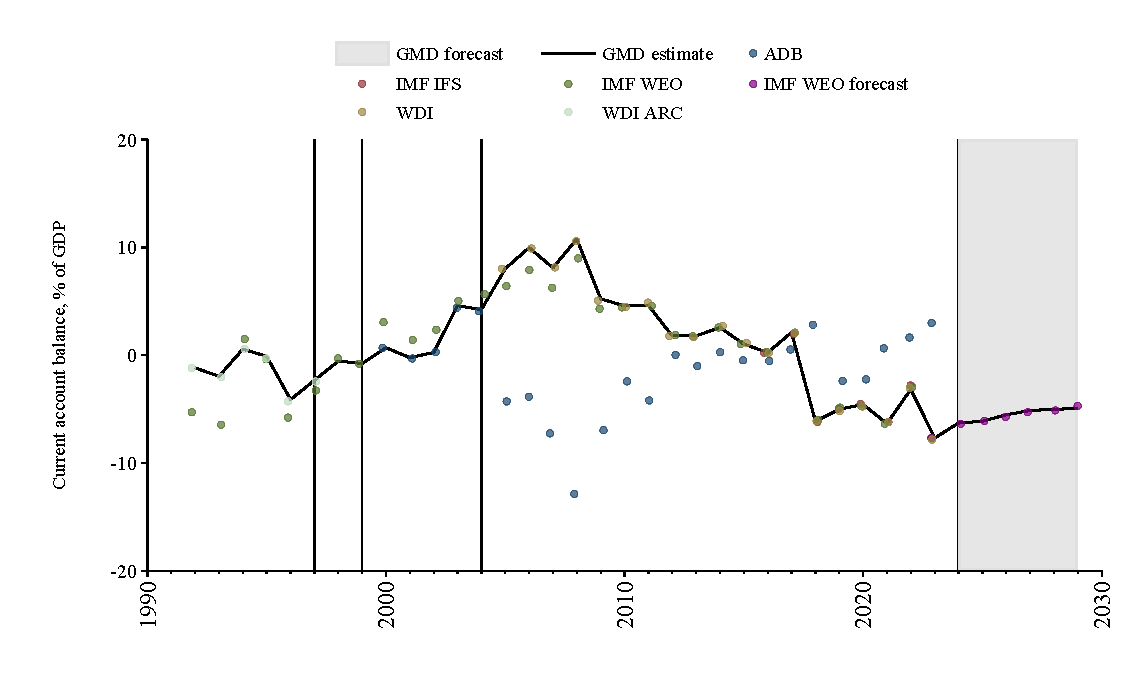
\includegraphics[width=\textwidth,height=0.6\textheight,keepaspectratio]{graphs/UZB_CA_GDP.pdf}
\end{figure}
\end{minipage}
\end{adjustbox}
\begin{adjustbox}{max totalsize={\paperwidth}{\paperheight},center}
\begin{minipage}[t][\textheight][t]{\textwidth}
\vspace*{0.5cm}
\phantomsection
\addcontentsline{toc}{section}{Consumer price index}
\begin{center}
{\Large\bfseries Consumer price index}
\end{center}
\vspace{0.5cm}
\begin{table}[H]
\centering
\small
\begin{tabular}{|l|l|l|}
\hline
\textbf{Source} & \textbf{Time span} & \textbf{Notes} \\
\hline
\rowcolor{white}\cite{WB_CC}& 1991 - 1999 &Spliced using overlapping data in 2000: (ratio = 0\%). \\
\rowcolor{lightgray}\cite{ADB}& 2000 - 2009 &Spliced using overlapping data in 2010: (ratio = 95.3\%). \\
\rowcolor{white}\cite{WDI}& 2010 - 2024 &Baseline source, overlaps with base year 2018. \\
\rowcolor{lightgray}\cite{IMF_WEO_forecast}& 2025 - 2029 &Spliced using overlapping data in 2030: (ratio = 319.3\%). \\
\hline
\end{tabular}
\end{table}
\begin{figure}[H]
\centering
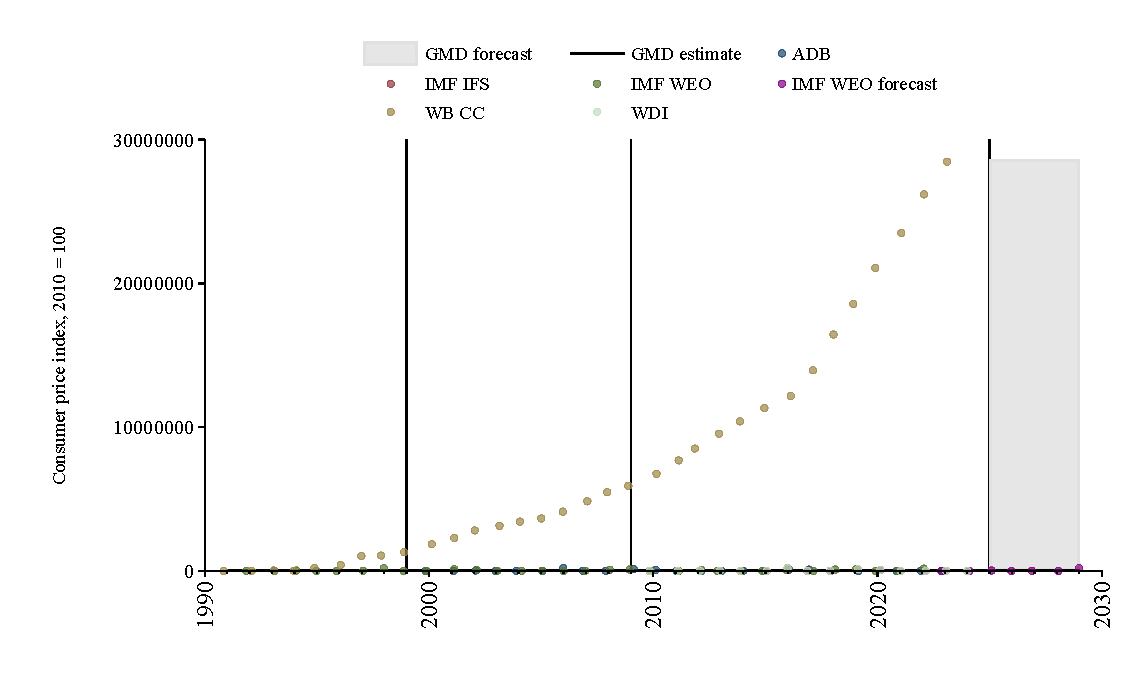
\includegraphics[width=\textwidth,height=0.6\textheight,keepaspectratio]{graphs/UZB_CPI.pdf}
\end{figure}
\end{minipage}
\end{adjustbox}
\begin{adjustbox}{max totalsize={\paperwidth}{\paperheight},center}
\begin{minipage}[t][\textheight][t]{\textwidth}
\vspace*{0.5cm}
\phantomsection
\addcontentsline{toc}{section}{Money supply (M0)}
\begin{center}
{\Large\bfseries Money supply (M0)}
\end{center}
\vspace{0.5cm}
\begin{table}[H]
\centering
\small
\begin{tabular}{|l|l|l|}
\hline
\textbf{Source} & \textbf{Time span} & \textbf{Notes} \\
\hline
\rowcolor{white}\cite{ADB}& 2000 - 2019 &Baseline source, overlaps with base year 2018. \\
\hline
\end{tabular}
\end{table}
\begin{figure}[H]
\centering
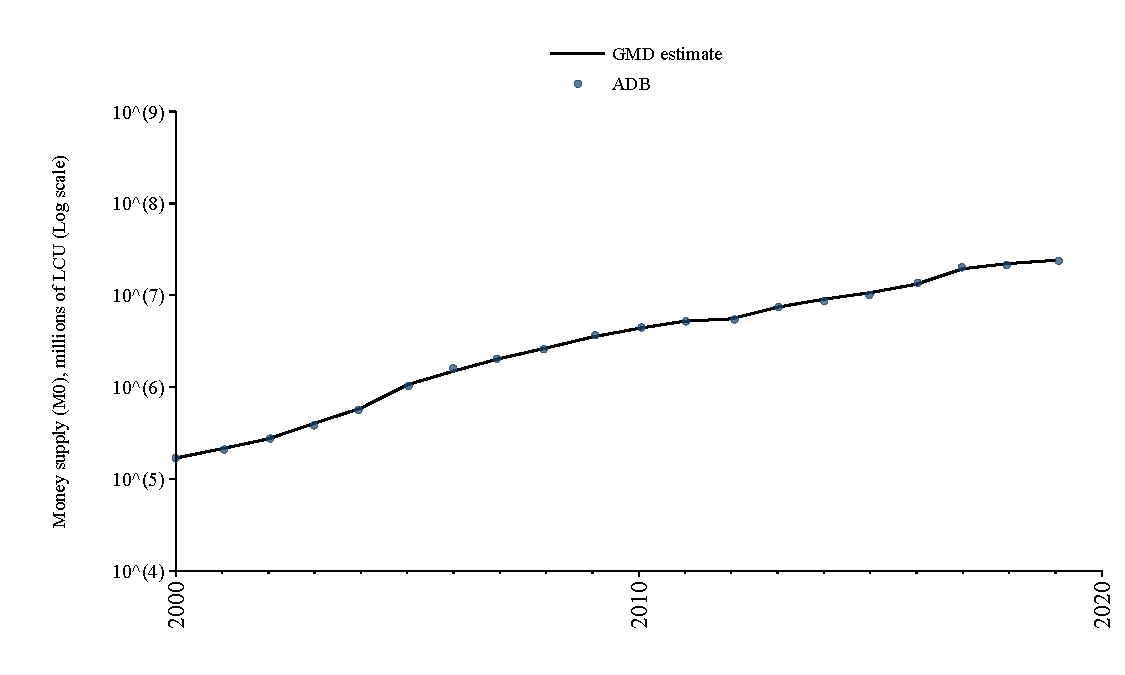
\includegraphics[width=\textwidth,height=0.6\textheight,keepaspectratio]{graphs/UZB_M0.pdf}
\end{figure}
\end{minipage}
\end{adjustbox}
\begin{adjustbox}{max totalsize={\paperwidth}{\paperheight},center}
\begin{minipage}[t][\textheight][t]{\textwidth}
\vspace*{0.5cm}
\phantomsection
\addcontentsline{toc}{section}{Money supply (M1)}
\begin{center}
{\Large\bfseries Money supply (M1)}
\end{center}
\vspace{0.5cm}
\begin{table}[H]
\centering
\small
\begin{tabular}{|l|l|l|}
\hline
\textbf{Source} & \textbf{Time span} & \textbf{Notes} \\
\hline
\rowcolor{white}\cite{ADB}& 2000 - 2019 &Baseline source, overlaps with base year 2018. \\
\hline
\end{tabular}
\end{table}
\begin{figure}[H]
\centering
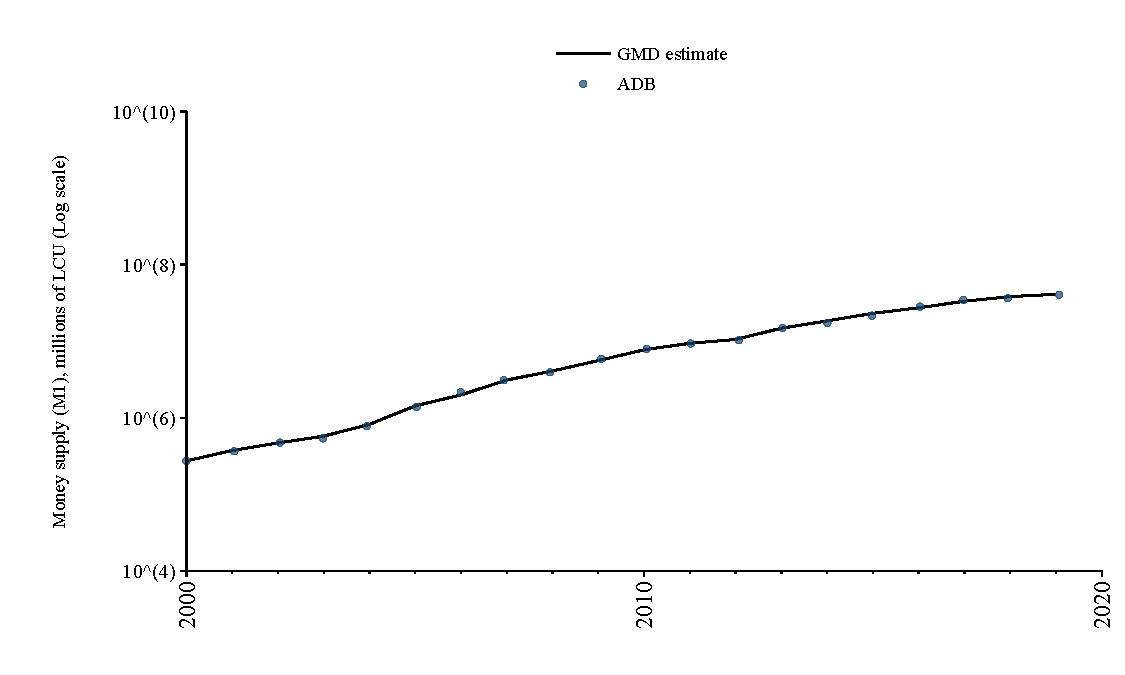
\includegraphics[width=\textwidth,height=0.6\textheight,keepaspectratio]{graphs/UZB_M1.pdf}
\end{figure}
\end{minipage}
\end{adjustbox}
\begin{adjustbox}{max totalsize={\paperwidth}{\paperheight},center}
\begin{minipage}[t][\textheight][t]{\textwidth}
\vspace*{0.5cm}
\phantomsection
\addcontentsline{toc}{section}{Money supply (M2)}
\begin{center}
{\Large\bfseries Money supply (M2)}
\end{center}
\vspace{0.5cm}
\begin{table}[H]
\centering
\small
\begin{tabular}{|l|l|l|}
\hline
\textbf{Source} & \textbf{Time span} & \textbf{Notes} \\
\hline
\rowcolor{white}\cite{ADB}& 2000 - 2019 &Baseline source, overlaps with base year 2018. \\
\hline
\end{tabular}
\end{table}
\begin{figure}[H]
\centering
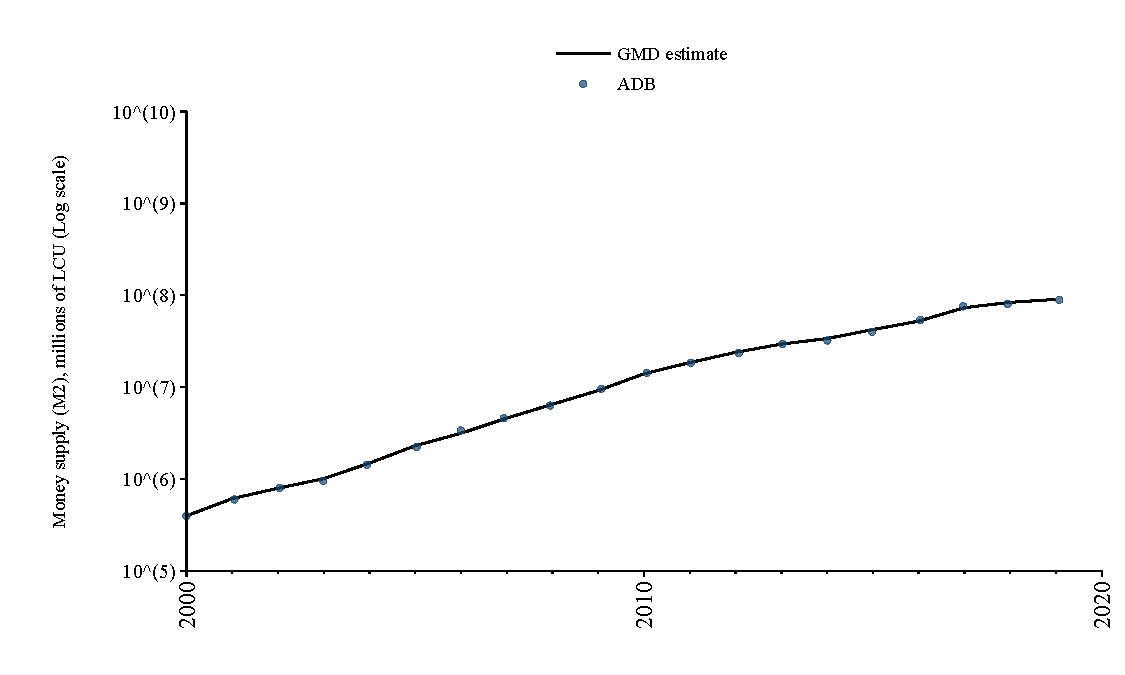
\includegraphics[width=\textwidth,height=0.6\textheight,keepaspectratio]{graphs/UZB_M2.pdf}
\end{figure}
\end{minipage}
\end{adjustbox}
\begin{adjustbox}{max totalsize={\paperwidth}{\paperheight},center}
\begin{minipage}[t][\textheight][t]{\textwidth}
\vspace*{0.5cm}
\phantomsection
\addcontentsline{toc}{section}{Real effective exchange rate}
\begin{center}
{\Large\bfseries Real effective exchange rate}
\end{center}
\vspace{0.5cm}
\begin{table}[H]
\centering
\small
\begin{tabular}{|l|l|l|}
\hline
\textbf{Source} & \textbf{Time span} & \textbf{Notes} \\
\hline
\rowcolor{white}\cite{BRUEGEL}& 1990 - 2023 &Baseline source, overlaps with base year 2018. \\
\hline
\end{tabular}
\end{table}
\begin{figure}[H]
\centering
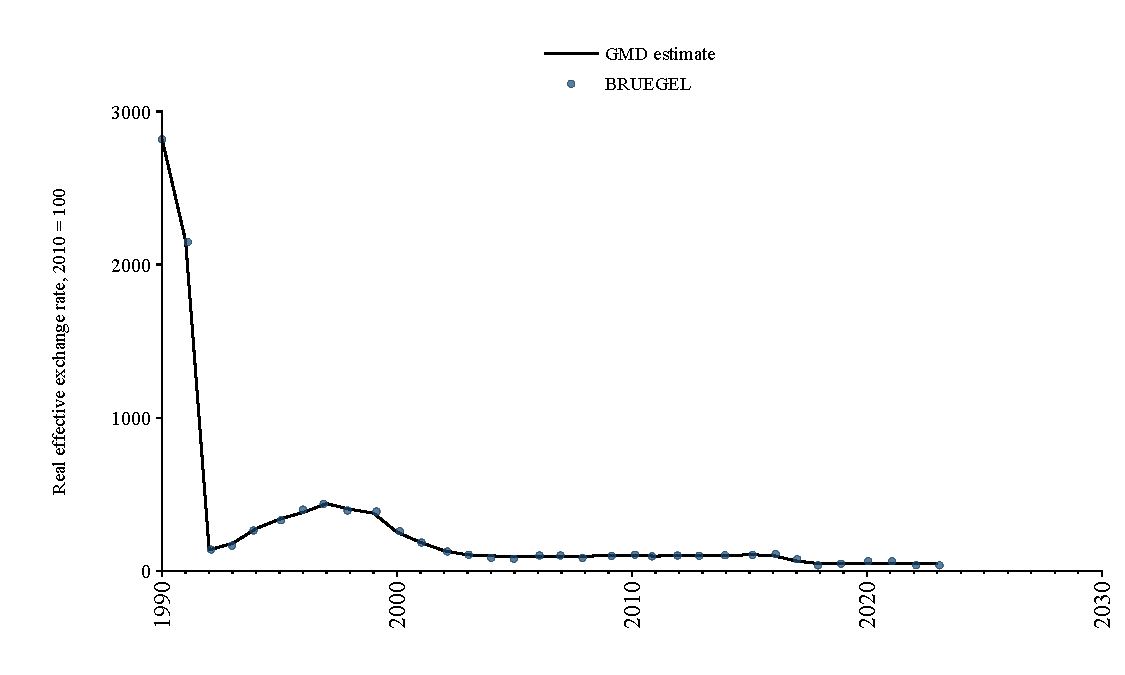
\includegraphics[width=\textwidth,height=0.6\textheight,keepaspectratio]{graphs/UZB_REER.pdf}
\end{figure}
\end{minipage}
\end{adjustbox}
\begin{adjustbox}{max totalsize={\paperwidth}{\paperheight},center}
\begin{minipage}[t][\textheight][t]{\textwidth}
\vspace*{0.5cm}
\phantomsection
\addcontentsline{toc}{section}{USD exchange rate}
\begin{center}
{\Large\bfseries USD exchange rate}
\end{center}
\vspace{0.5cm}
\begin{table}[H]
\centering
\small
\begin{tabular}{|l|l|l|}
\hline
\textbf{Source} & \textbf{Time span} & \textbf{Notes} \\
\hline
\rowcolor{white}\cite{PWT}& 1990 - 1993 &Spliced using overlapping data in 1994. \\
\rowcolor{lightgray}\cite{BIS}& 1994 - 2024 &Baseline source, overlaps with base year 2018. \\
\hline
\end{tabular}
\end{table}
\begin{figure}[H]
\centering
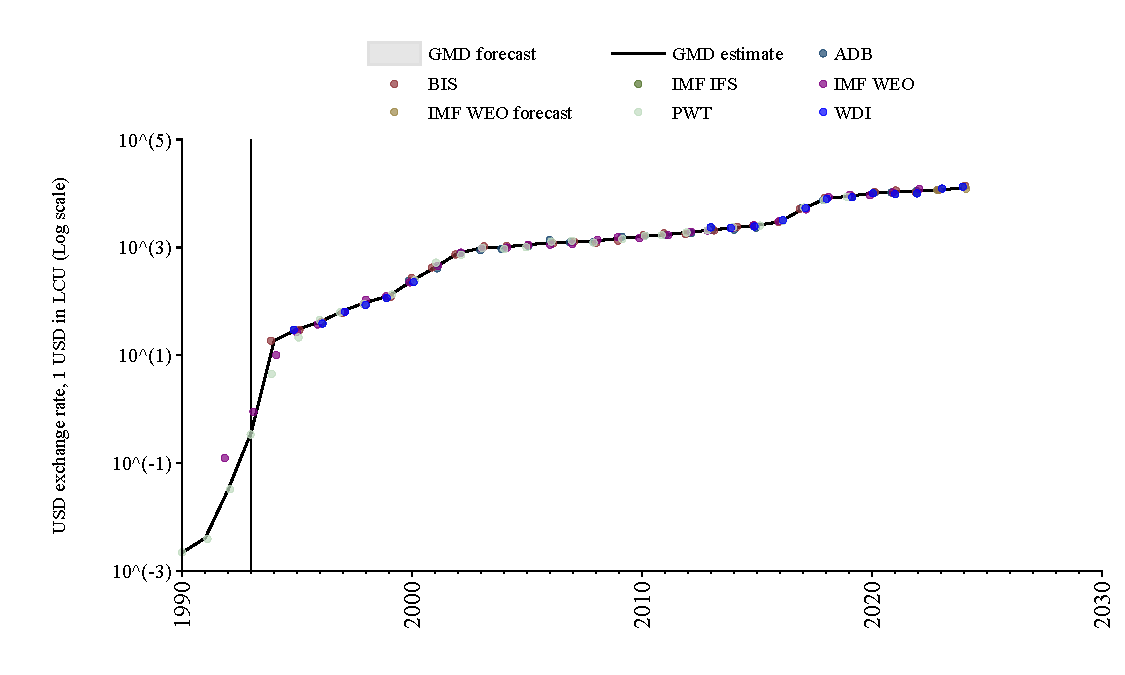
\includegraphics[width=\textwidth,height=0.6\textheight,keepaspectratio]{graphs/UZB_USDfx.pdf}
\end{figure}
\end{minipage}
\end{adjustbox}
\begin{adjustbox}{max totalsize={\paperwidth}{\paperheight},center}
\begin{minipage}[t][\textheight][t]{\textwidth}
\vspace*{0.5cm}
\phantomsection
\addcontentsline{toc}{section}{Central bank policy rate}
\begin{center}
{\Large\bfseries Central bank policy rate}
\end{center}
\vspace{0.5cm}
\begin{table}[H]
\centering
\small
\begin{tabular}{|l|l|l|}
\hline
\textbf{Source} & \textbf{Time span} & \textbf{Notes} \\
\hline
\rowcolor{white}\cite{Grimm}& 2013 - 2022 &Baseline source, overlaps with base year 2018. \\
\rowcolor{lightgray}\cite{IMF_IFS}& 2023 - 2024 &Spliced using overlapping data in 2025. \\
\hline
\end{tabular}
\end{table}
\begin{figure}[H]
\centering
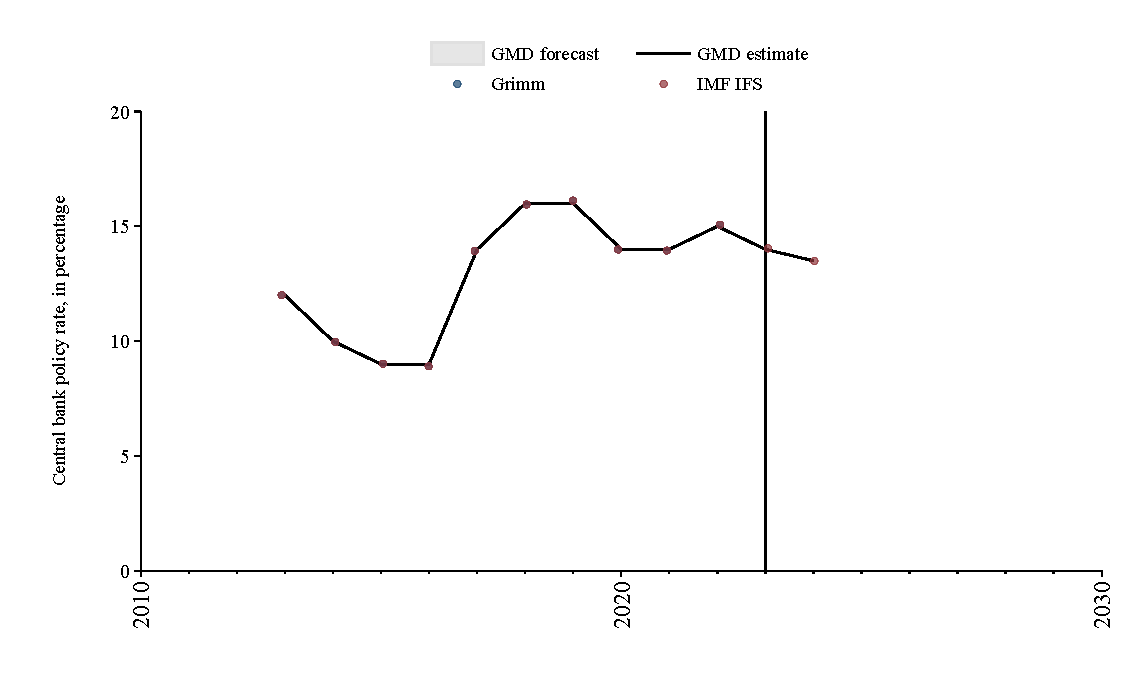
\includegraphics[width=\textwidth,height=0.6\textheight,keepaspectratio]{graphs/UZB_cbrate.pdf}
\end{figure}
\end{minipage}
\end{adjustbox}
\begin{adjustbox}{max totalsize={\paperwidth}{\paperheight},center}
\begin{minipage}[t][\textheight][t]{\textwidth}
\vspace*{0.5cm}
\phantomsection
\addcontentsline{toc}{section}{Total consumption}
\begin{center}
{\Large\bfseries Total consumption}
\end{center}
\vspace{0.5cm}
\begin{table}[H]
\centering
\small
\begin{tabular}{|l|l|l|}
\hline
\textbf{Source} & \textbf{Time span} & \textbf{Notes} \\
\hline
\rowcolor{white}\cite{WDI_ARC}& 1987 - 1989 &Spliced using overlapping data in 1990: (ratio = 86.3\%). \\
\rowcolor{lightgray}\cite{UN}& 1990 - 1991 &Spliced using overlapping data in 1992: (ratio = 67.2\%). \\
\rowcolor{white}\cite{WDI}& 1992 - 2023 &Baseline source, overlaps with base year 2018. \\
\hline
\end{tabular}
\end{table}
\begin{figure}[H]
\centering
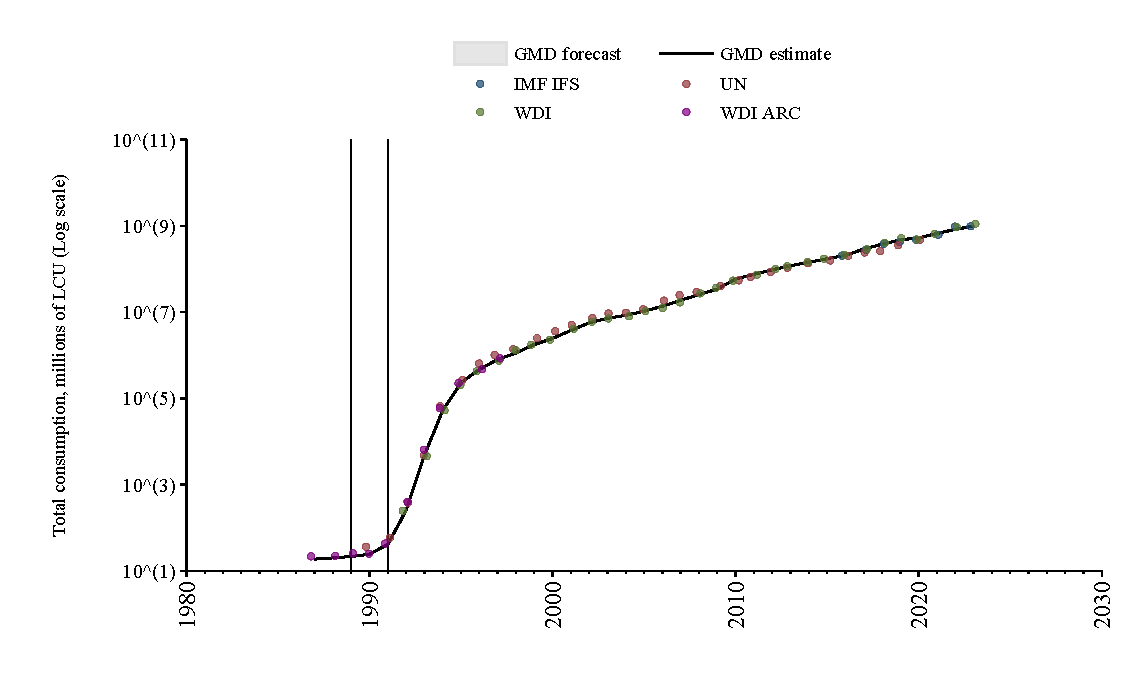
\includegraphics[width=\textwidth,height=0.6\textheight,keepaspectratio]{graphs/UZB_cons.pdf}
\end{figure}
\end{minipage}
\end{adjustbox}
\begin{adjustbox}{max totalsize={\paperwidth}{\paperheight},center}
\begin{minipage}[t][\textheight][t]{\textwidth}
\vspace*{0.5cm}
\phantomsection
\addcontentsline{toc}{section}{Total consumption to GDP ratio}
\begin{center}
{\Large\bfseries Total consumption to GDP ratio}
\end{center}
\vspace{0.5cm}
\begin{table}[H]
\centering
\small
\begin{tabular}{|l|l|l|}
\hline
\textbf{Source} & \textbf{Time span} & \textbf{Notes} \\
\hline
\rowcolor{white}\cite{WDI_ARC}& 1987 - 1991 &Spliced using overlapping data in 1992. \\
\rowcolor{lightgray}\cite{WDI}& 1992 - 2023 &Baseline source, overlaps with base year 2018. \\
\hline
\end{tabular}
\end{table}
\begin{figure}[H]
\centering
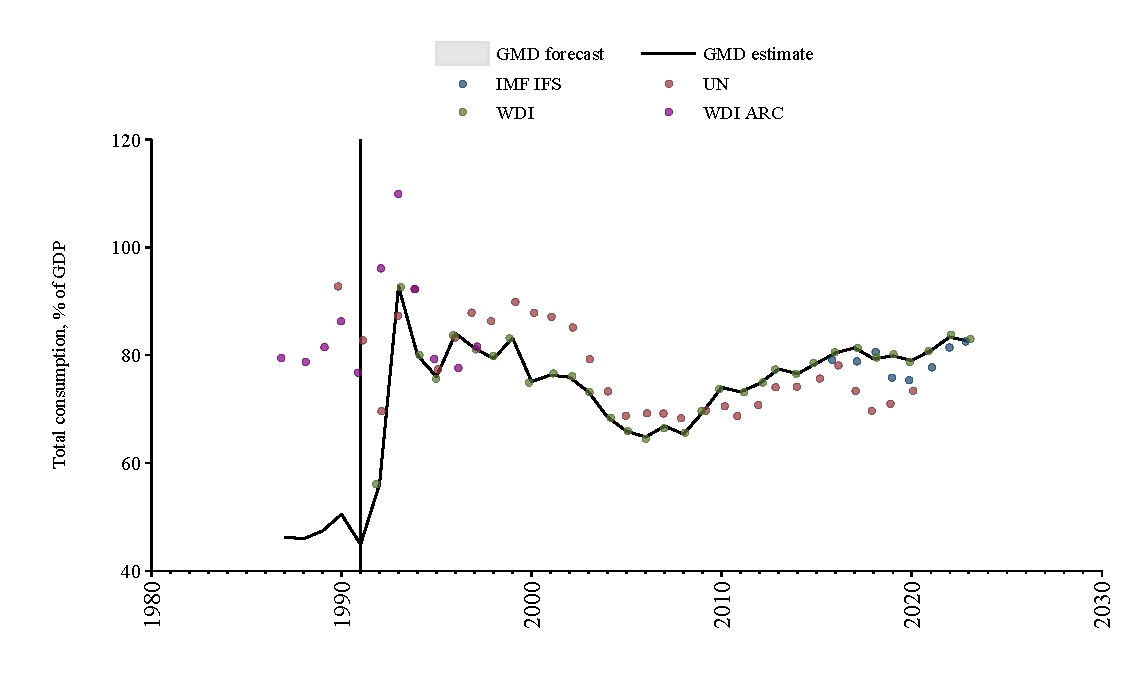
\includegraphics[width=\textwidth,height=0.6\textheight,keepaspectratio]{graphs/UZB_cons_GDP.pdf}
\end{figure}
\end{minipage}
\end{adjustbox}
\begin{adjustbox}{max totalsize={\paperwidth}{\paperheight},center}
\begin{minipage}[t][\textheight][t]{\textwidth}
\vspace*{0.5cm}
\phantomsection
\addcontentsline{toc}{section}{Exports}
\begin{center}
{\Large\bfseries Exports}
\end{center}
\vspace{0.5cm}
\begin{table}[H]
\centering
\small
\begin{tabular}{|l|l|l|}
\hline
\textbf{Source} & \textbf{Time span} & \textbf{Notes} \\
\hline
\rowcolor{white}\cite{UN}& 1990 - 1996 &Spliced using overlapping data in 1997: (ratio = 90.8\%). \\
\rowcolor{lightgray}\cite{WDI}& 1997 - 2023 &Baseline source, overlaps with base year 2018. \\
\rowcolor{white}\cite{IMF_WEO_forecast}& 2024 - 2029 &Spliced using overlapping data in 2030. \\
\hline
\end{tabular}
\end{table}
\begin{figure}[H]
\centering
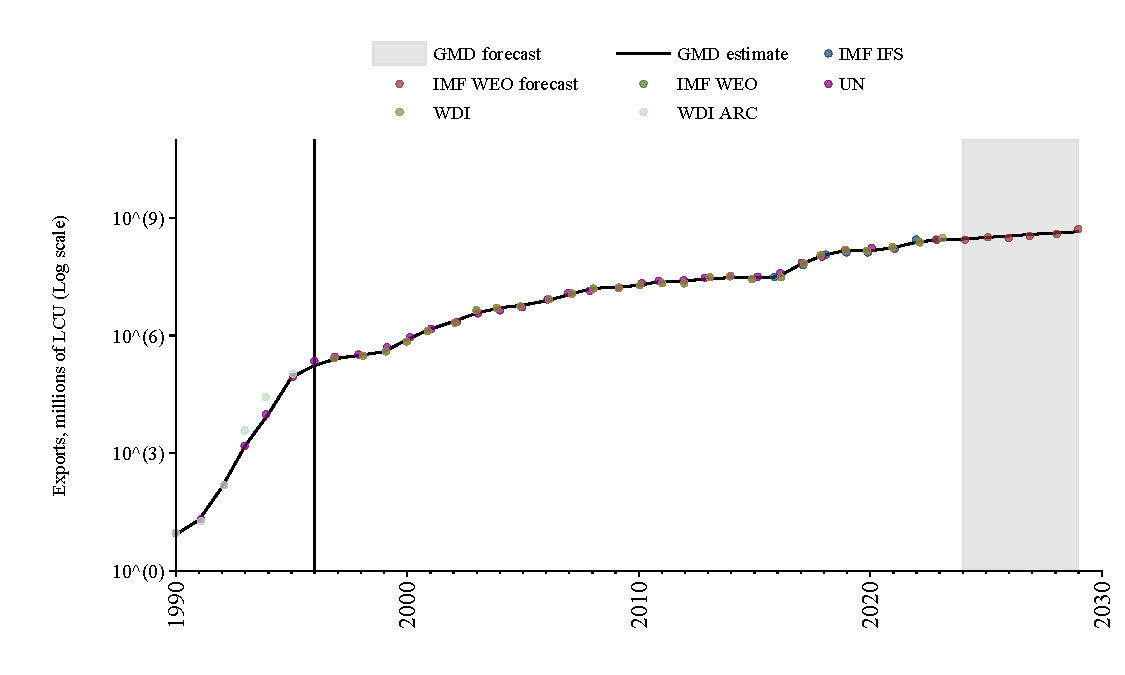
\includegraphics[width=\textwidth,height=0.6\textheight,keepaspectratio]{graphs/UZB_exports.pdf}
\end{figure}
\end{minipage}
\end{adjustbox}
\begin{adjustbox}{max totalsize={\paperwidth}{\paperheight},center}
\begin{minipage}[t][\textheight][t]{\textwidth}
\vspace*{0.5cm}
\phantomsection
\addcontentsline{toc}{section}{Exports to GDP ratio}
\begin{center}
{\Large\bfseries Exports to GDP ratio}
\end{center}
\vspace{0.5cm}
\begin{table}[H]
\centering
\small
\begin{tabular}{|l|l|l|}
\hline
\textbf{Source} & \textbf{Time span} & \textbf{Notes} \\
\hline
\rowcolor{white}\cite{UN}& 1990 - 2020 &Baseline source, overlaps with base year 2018. \\
\rowcolor{lightgray}\cite{WDI}& 2021 - 2023 &Spliced using overlapping data in 2024: (ratio = 120.1\%). \\
\rowcolor{white}\cite{IMF_WEO_forecast}& 2024 - 2029 &Spliced using overlapping data in 2030: (ratio = 120.1\%). \\
\hline
\end{tabular}
\end{table}
\begin{figure}[H]
\centering
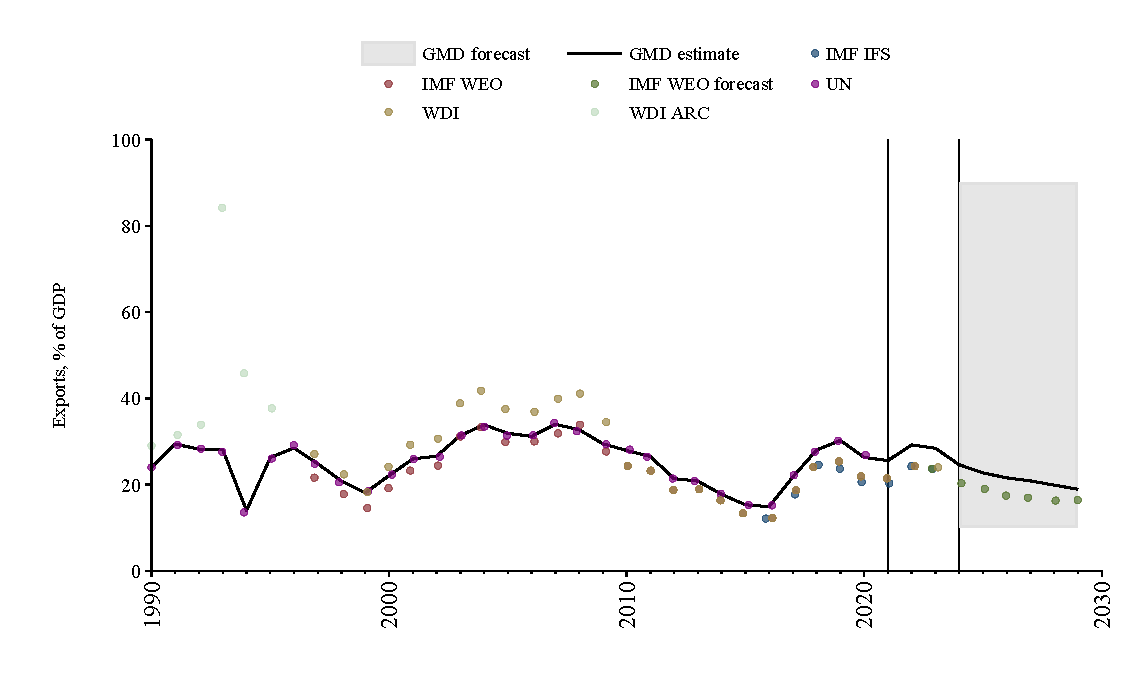
\includegraphics[width=\textwidth,height=0.6\textheight,keepaspectratio]{graphs/UZB_exports_GDP.pdf}
\end{figure}
\end{minipage}
\end{adjustbox}
\begin{adjustbox}{max totalsize={\paperwidth}{\paperheight},center}
\begin{minipage}[t][\textheight][t]{\textwidth}
\vspace*{0.5cm}
\phantomsection
\addcontentsline{toc}{section}{Fixed investment}
\begin{center}
{\Large\bfseries Fixed investment}
\end{center}
\vspace{0.5cm}
\begin{table}[H]
\centering
\small
\begin{tabular}{|l|l|l|}
\hline
\textbf{Source} & \textbf{Time span} & \textbf{Notes} \\
\hline
\rowcolor{white}\cite{WDI_ARC}& 1987 - 1989 &Spliced using overlapping data in 1990: (ratio = 166.7\%). \\
\rowcolor{lightgray}\cite{UN}& 1990 - 1991 &Spliced using overlapping data in 1992: (ratio = 144.7\%). \\
\rowcolor{white}\cite{WDI}& 1992 - 2023 &Baseline source, overlaps with base year 2018. \\
\hline
\end{tabular}
\end{table}
\begin{figure}[H]
\centering
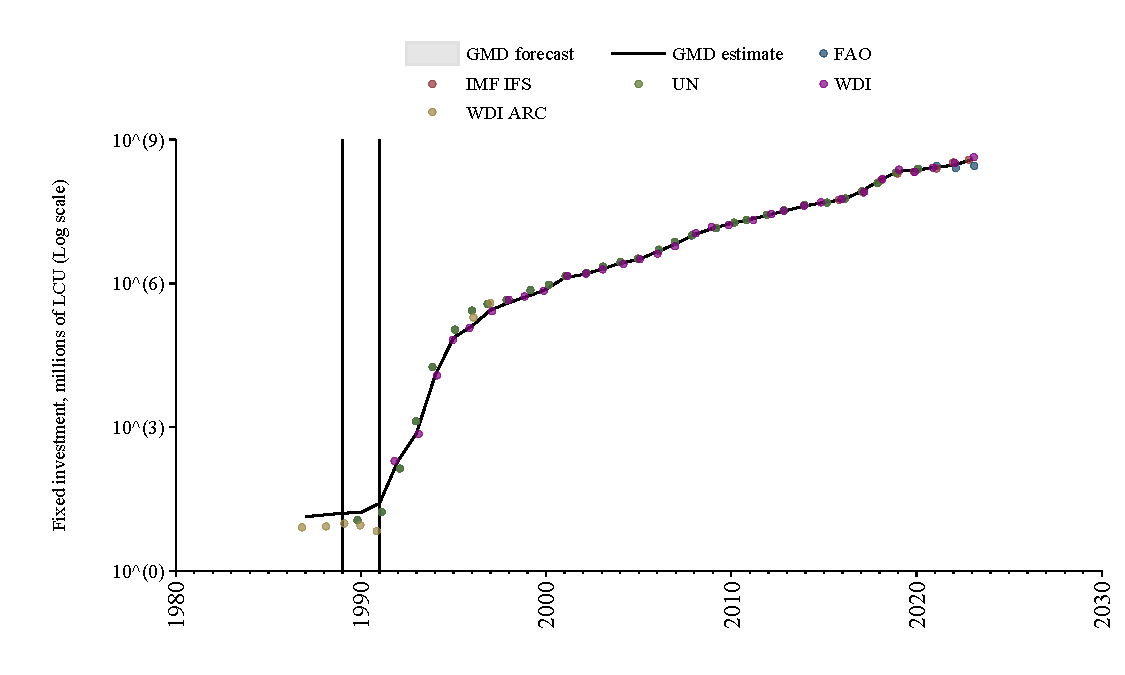
\includegraphics[width=\textwidth,height=0.6\textheight,keepaspectratio]{graphs/UZB_finv.pdf}
\end{figure}
\end{minipage}
\end{adjustbox}
\begin{adjustbox}{max totalsize={\paperwidth}{\paperheight},center}
\begin{minipage}[t][\textheight][t]{\textwidth}
\vspace*{0.5cm}
\phantomsection
\addcontentsline{toc}{section}{Fixed investment to GDP ratio}
\begin{center}
{\Large\bfseries Fixed investment to GDP ratio}
\end{center}
\vspace{0.5cm}
\begin{table}[H]
\centering
\small
\begin{tabular}{|l|l|l|}
\hline
\textbf{Source} & \textbf{Time span} & \textbf{Notes} \\
\hline
\rowcolor{white}\cite{WDI_ARC}& 1987 - 1989 &Spliced using overlapping data in 1990: (ratio = 166.5\%). \\
\rowcolor{lightgray}\cite{UN}& 1990 - 1991 &Spliced using overlapping data in 1992: (ratio = 173.8\%). \\
\rowcolor{white}\cite{WDI}& 1992 - 2023 &Baseline source, overlaps with base year 2018. \\
\hline
\end{tabular}
\end{table}
\begin{figure}[H]
\centering
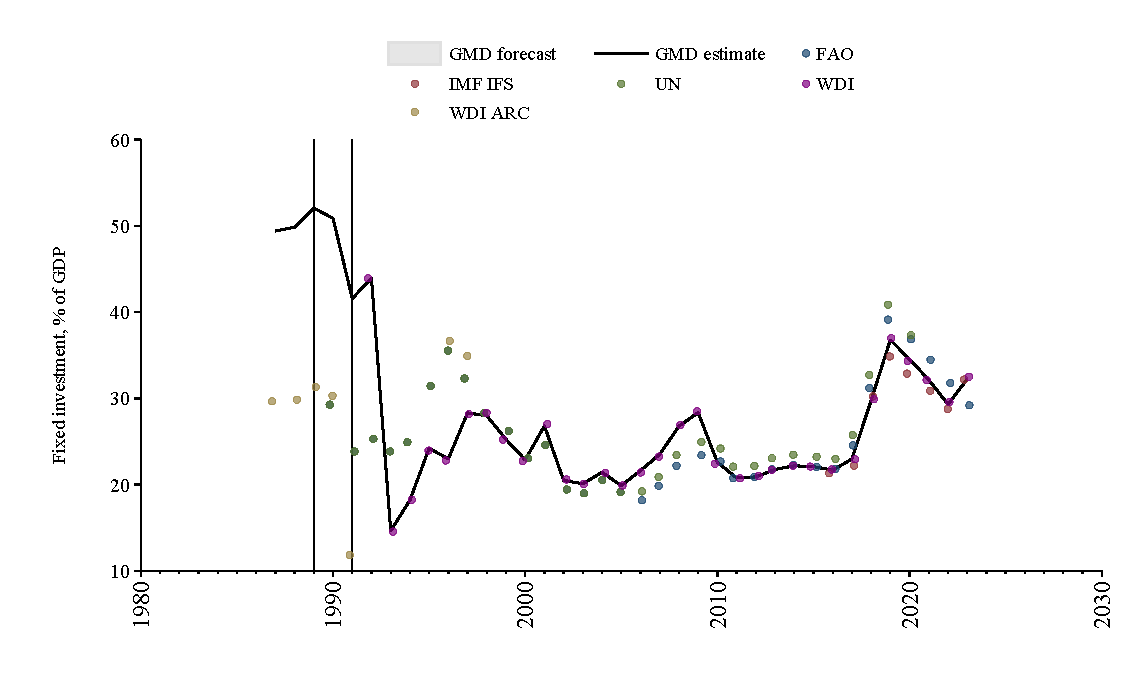
\includegraphics[width=\textwidth,height=0.6\textheight,keepaspectratio]{graphs/UZB_finv_GDP.pdf}
\end{figure}
\end{minipage}
\end{adjustbox}
\begin{adjustbox}{max totalsize={\paperwidth}{\paperheight},center}
\begin{minipage}[t][\textheight][t]{\textwidth}
\vspace*{0.5cm}
\phantomsection
\addcontentsline{toc}{section}{Government debt}
\begin{center}
{\Large\bfseries Government debt}
\end{center}
\vspace{0.5cm}
\begin{table}[H]
\centering
\small
\begin{tabular}{|l|l|l|}
\hline
\textbf{Source} & \textbf{Time span} & \textbf{Notes} \\
\hline
\rowcolor{white}\cite{IMF_FPP}& 1997 - 2023 &Baseline source, overlaps with base year 2018. Data refers to general government.\\
\rowcolor{lightgray}\cite{IMF_WEO_forecast}& 2024 - 2029 &Spliced using overlapping data in 2030. \\
\hline
\end{tabular}
\end{table}
\begin{figure}[H]
\centering
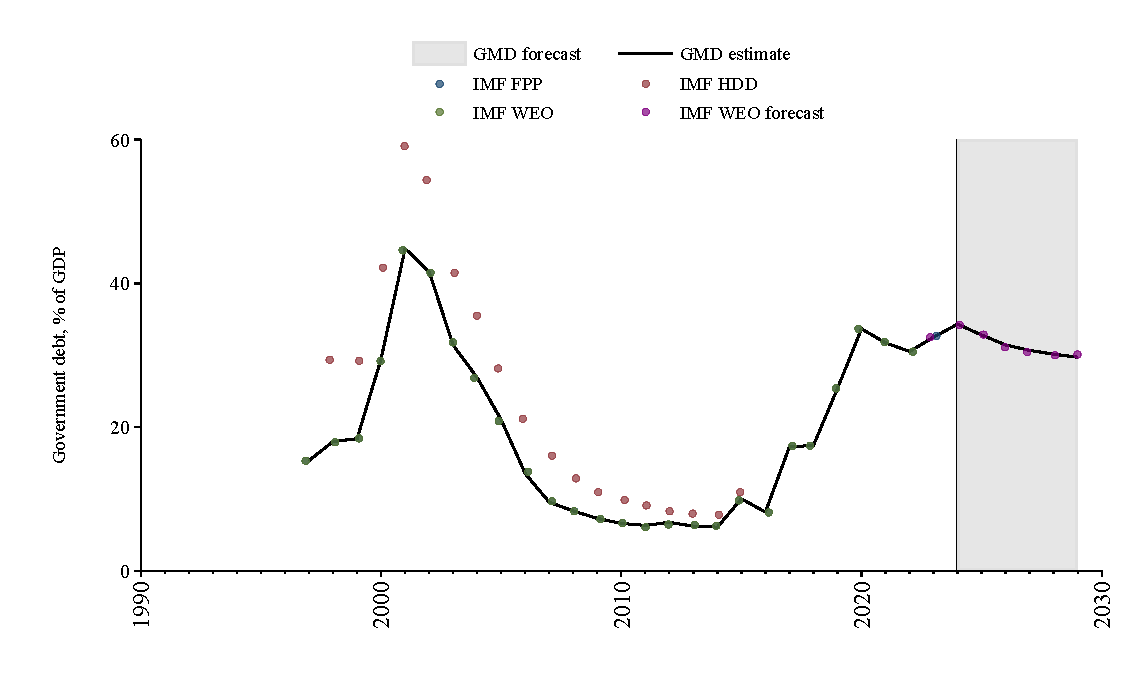
\includegraphics[width=\textwidth,height=0.6\textheight,keepaspectratio]{graphs/UZB_govdebt_GDP.pdf}
\end{figure}
\end{minipage}
\end{adjustbox}
\begin{adjustbox}{max totalsize={\paperwidth}{\paperheight},center}
\begin{minipage}[t][\textheight][t]{\textwidth}
\vspace*{0.5cm}
\phantomsection
\addcontentsline{toc}{section}{Government deficit}
\begin{center}
{\Large\bfseries Government deficit}
\end{center}
\vspace{0.5cm}
\begin{table}[H]
\centering
\small
\begin{tabular}{|l|l|l|}
\hline
\textbf{Source} & \textbf{Time span} & \textbf{Notes} \\
\hline
\rowcolor{white}\cite{IMF_WEO}& 1992 - 2022 &Baseline source, overlaps with base year 2018. \\
\rowcolor{lightgray}\cite{IMF_FPP}& 2023 - 2023 &Spliced using overlapping data in 2024. \\
\rowcolor{white}\cite{IMF_WEO_forecast}& 2024 - 2029 &Spliced using overlapping data in 2030. \\
\hline
\end{tabular}
\end{table}
\begin{figure}[H]
\centering
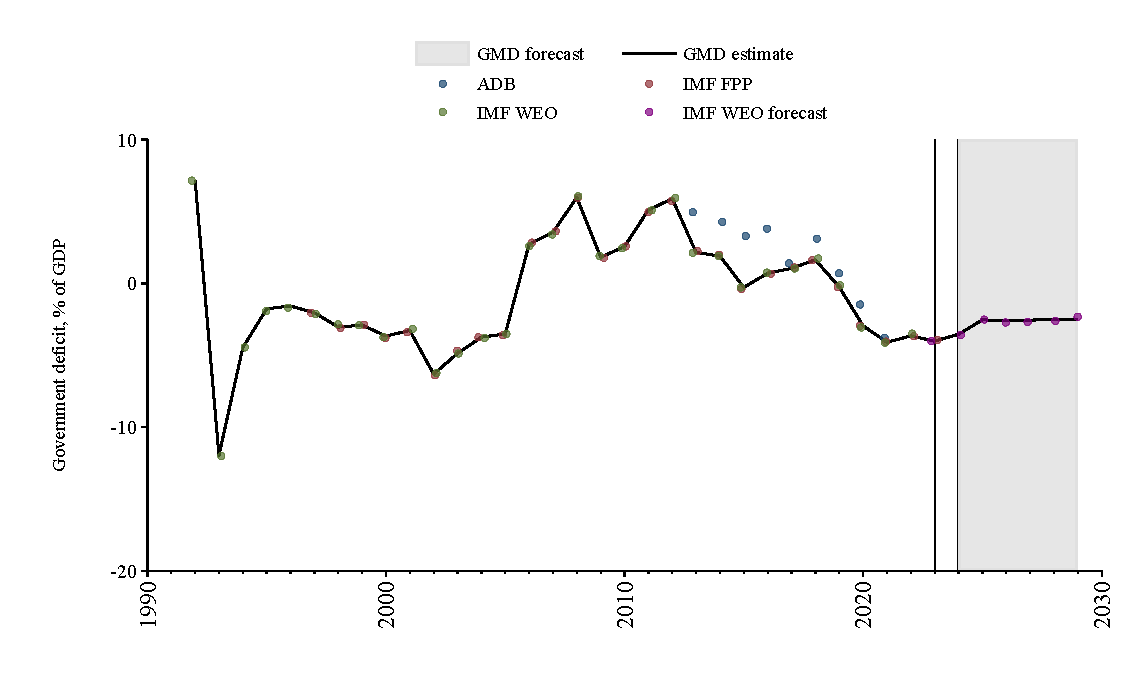
\includegraphics[width=\textwidth,height=0.6\textheight,keepaspectratio]{graphs/UZB_govdef_GDP.pdf}
\end{figure}
\end{minipage}
\end{adjustbox}
\begin{adjustbox}{max totalsize={\paperwidth}{\paperheight},center}
\begin{minipage}[t][\textheight][t]{\textwidth}
\vspace*{0.5cm}
\phantomsection
\addcontentsline{toc}{section}{Government expenditure}
\begin{center}
{\Large\bfseries Government expenditure}
\end{center}
\vspace{0.5cm}
\begin{table}[H]
\centering
\small
\begin{tabular}{|l|l|l|}
\hline
\textbf{Source} & \textbf{Time span} & \textbf{Notes} \\
\hline
\rowcolor{white}\cite{GMD_estimated}& 1992 - 2029 &Baseline source, overlaps with base year 2018. \\
\hline
\end{tabular}
\end{table}
\begin{figure}[H]
\centering
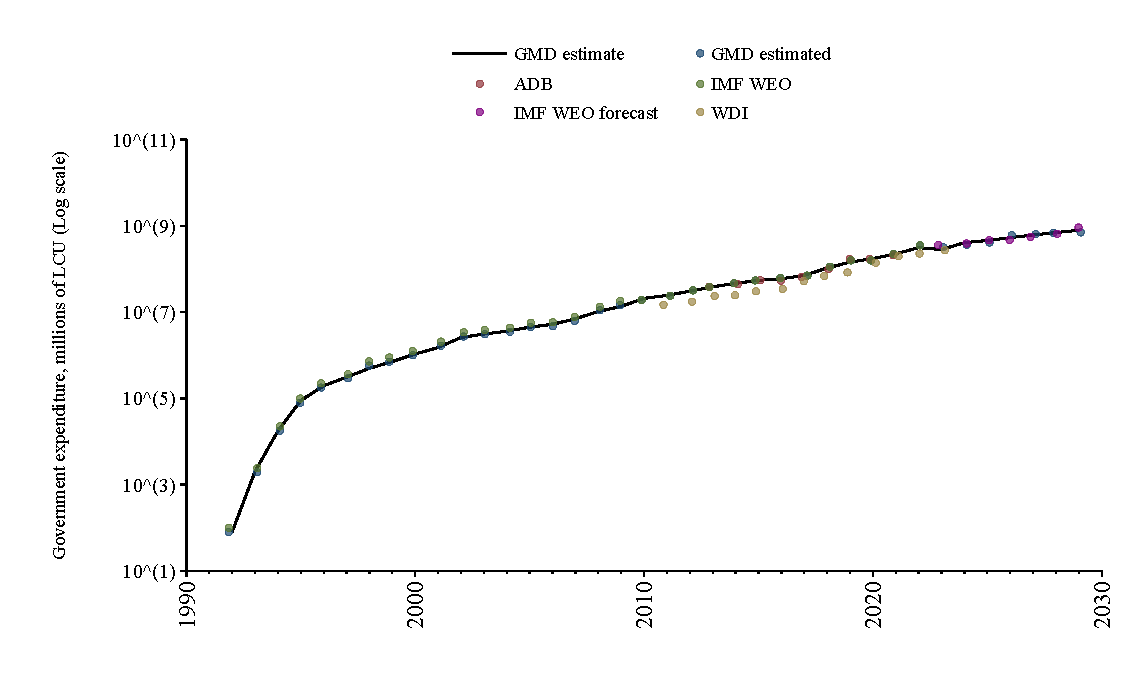
\includegraphics[width=\textwidth,height=0.6\textheight,keepaspectratio]{graphs/UZB_govexp.pdf}
\end{figure}
\end{minipage}
\end{adjustbox}
\begin{adjustbox}{max totalsize={\paperwidth}{\paperheight},center}
\begin{minipage}[t][\textheight][t]{\textwidth}
\vspace*{0.5cm}
\phantomsection
\addcontentsline{toc}{section}{Government expenditure to GDP ratio}
\begin{center}
{\Large\bfseries Government expenditure to GDP ratio}
\end{center}
\vspace{0.5cm}
\begin{table}[H]
\centering
\small
\begin{tabular}{|l|l|l|}
\hline
\textbf{Source} & \textbf{Time span} & \textbf{Notes} \\
\hline
\rowcolor{white}\cite{IMF_WEO}& 1992 - 2022 &Baseline source, overlaps with base year 2018. Data refers to general government.\\
\rowcolor{lightgray}\cite{WDI}& 2023 - 2023 &Spliced using overlapping data in 2024. Data refers to general government.\\
\rowcolor{white}\cite{IMF_WEO_forecast}& 2024 - 2029 &Spliced using overlapping data in 2030. \\
\hline
\end{tabular}
\end{table}
\begin{figure}[H]
\centering
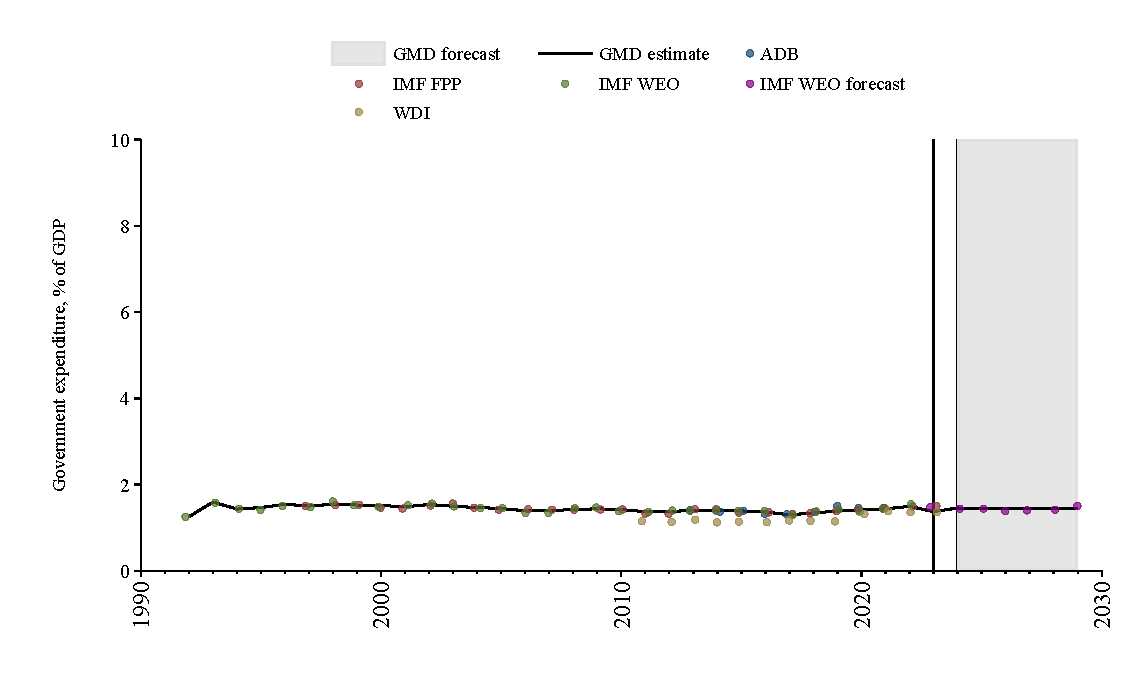
\includegraphics[width=\textwidth,height=0.6\textheight,keepaspectratio]{graphs/UZB_govexp_GDP.pdf}
\end{figure}
\end{minipage}
\end{adjustbox}
\begin{adjustbox}{max totalsize={\paperwidth}{\paperheight},center}
\begin{minipage}[t][\textheight][t]{\textwidth}
\vspace*{0.5cm}
\phantomsection
\addcontentsline{toc}{section}{Government revenue}
\begin{center}
{\Large\bfseries Government revenue}
\end{center}
\vspace{0.5cm}
\begin{table}[H]
\centering
\small
\begin{tabular}{|l|l|l|}
\hline
\textbf{Source} & \textbf{Time span} & \textbf{Notes} \\
\hline
\rowcolor{white}\cite{GMD_estimated}& 1992 - 2029 &Baseline source, overlaps with base year 2018. \\
\hline
\end{tabular}
\end{table}
\begin{figure}[H]
\centering
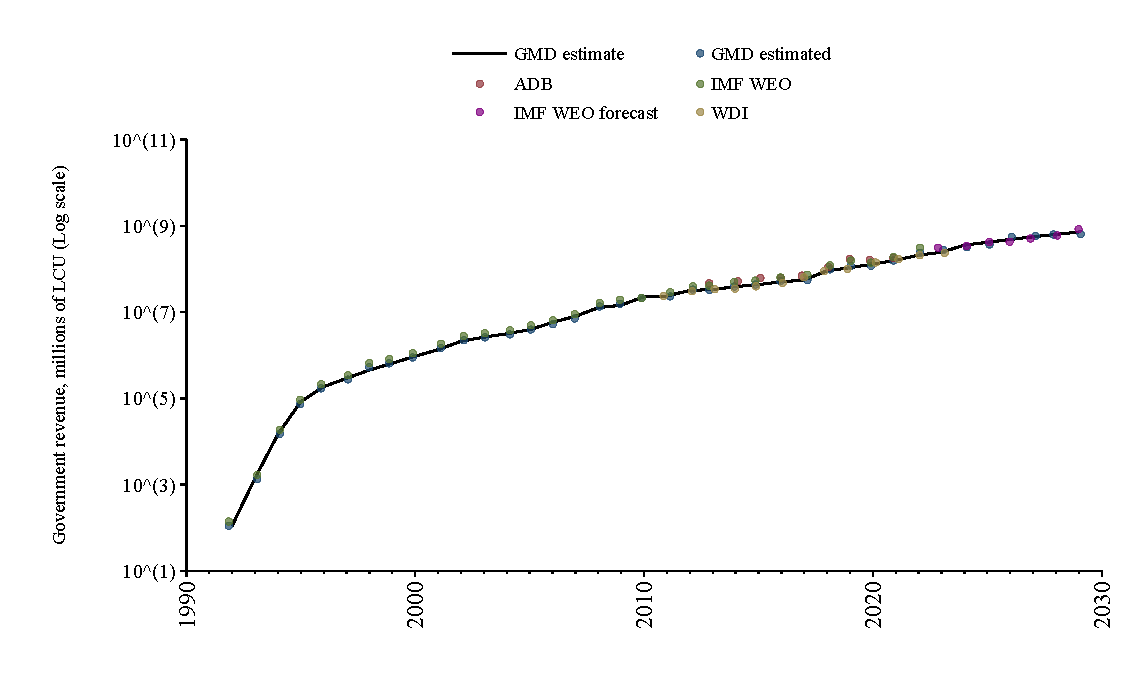
\includegraphics[width=\textwidth,height=0.6\textheight,keepaspectratio]{graphs/UZB_govrev.pdf}
\end{figure}
\end{minipage}
\end{adjustbox}
\begin{adjustbox}{max totalsize={\paperwidth}{\paperheight},center}
\begin{minipage}[t][\textheight][t]{\textwidth}
\vspace*{0.5cm}
\phantomsection
\addcontentsline{toc}{section}{Government revenue to GDP ratio}
\begin{center}
{\Large\bfseries Government revenue to GDP ratio}
\end{center}
\vspace{0.5cm}
\begin{table}[H]
\centering
\small
\begin{tabular}{|l|l|l|}
\hline
\textbf{Source} & \textbf{Time span} & \textbf{Notes} \\
\hline
\rowcolor{white}\cite{IMF_WEO}& 1992 - 2010 &Spliced using overlapping data in 2011. Data refers to general government.\\
\rowcolor{lightgray}\cite{WDI}& 2011 - 2023 &Baseline source, overlaps with base year 2018. Data refers to general government.\\
\rowcolor{white}\cite{IMF_WEO_forecast}& 2024 - 2029 &Spliced using overlapping data in 2030. \\
\hline
\end{tabular}
\end{table}
\begin{figure}[H]
\centering
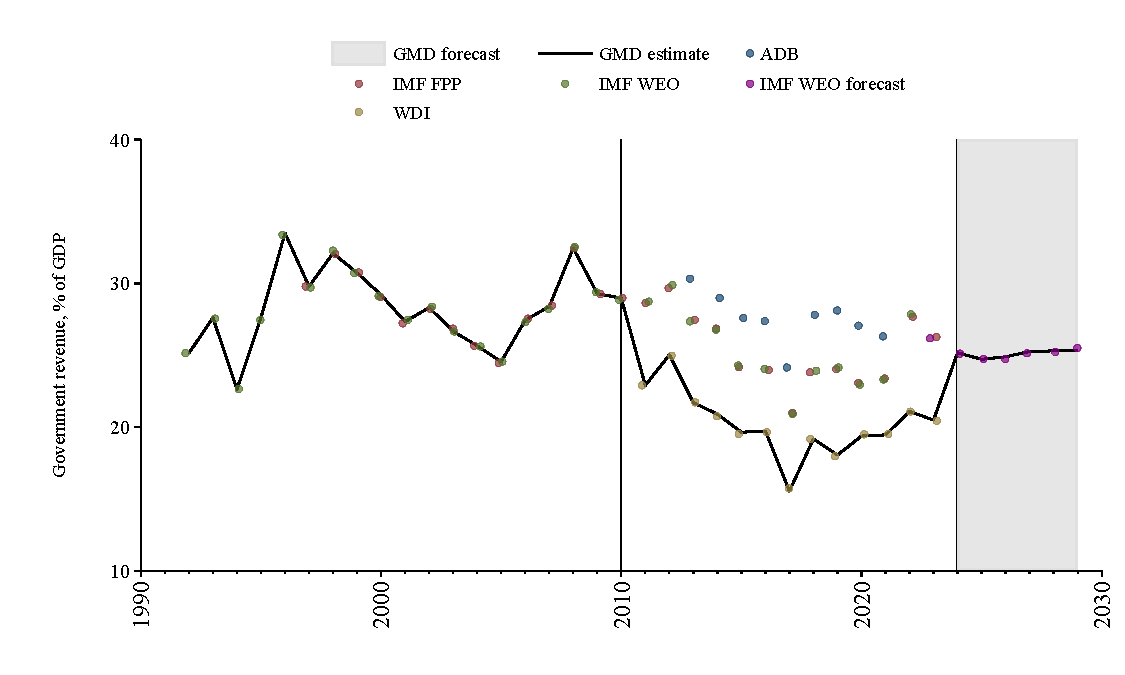
\includegraphics[width=\textwidth,height=0.6\textheight,keepaspectratio]{graphs/UZB_govrev_GDP.pdf}
\end{figure}
\end{minipage}
\end{adjustbox}
\begin{adjustbox}{max totalsize={\paperwidth}{\paperheight},center}
\begin{minipage}[t][\textheight][t]{\textwidth}
\vspace*{0.5cm}
\phantomsection
\addcontentsline{toc}{section}{Government tax revenue}
\begin{center}
{\Large\bfseries Government tax revenue}
\end{center}
\vspace{0.5cm}
\begin{table}[H]
\centering
\small
\begin{tabular}{|l|l|l|}
\hline
\textbf{Source} & \textbf{Time span} & \textbf{Notes} \\
\hline
\rowcolor{white}\cite{GMD_estimated}& 2011 - 2023 &Baseline source, overlaps with base year 2018. \\
\hline
\end{tabular}
\end{table}
\begin{figure}[H]
\centering
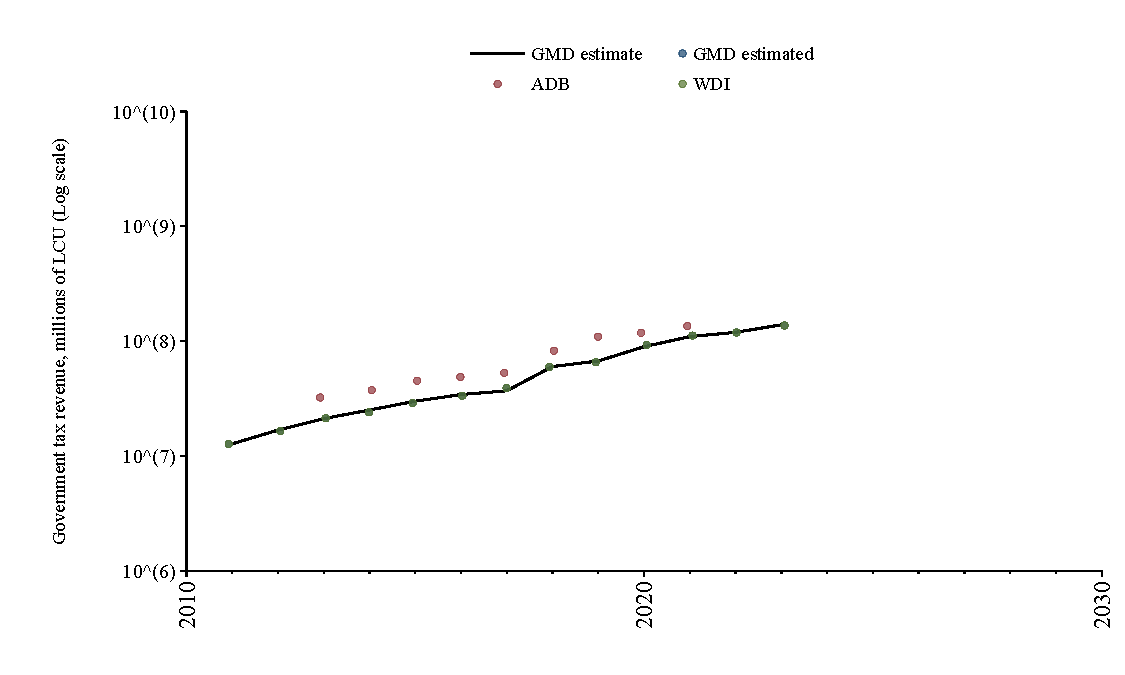
\includegraphics[width=\textwidth,height=0.6\textheight,keepaspectratio]{graphs/UZB_govtax.pdf}
\end{figure}
\end{minipage}
\end{adjustbox}
\begin{adjustbox}{max totalsize={\paperwidth}{\paperheight},center}
\begin{minipage}[t][\textheight][t]{\textwidth}
\vspace*{0.5cm}
\phantomsection
\addcontentsline{toc}{section}{Government tax revenue to GDP ratio}
\begin{center}
{\Large\bfseries Government tax revenue to GDP ratio}
\end{center}
\vspace{0.5cm}
\begin{table}[H]
\centering
\small
\begin{tabular}{|l|l|l|}
\hline
\textbf{Source} & \textbf{Time span} & \textbf{Notes} \\
\hline
\rowcolor{white}\cite{WDI}& 2011 - 2023 &Baseline source, overlaps with base year 2018. Data refers to central government.\\
\hline
\end{tabular}
\end{table}
\begin{figure}[H]
\centering
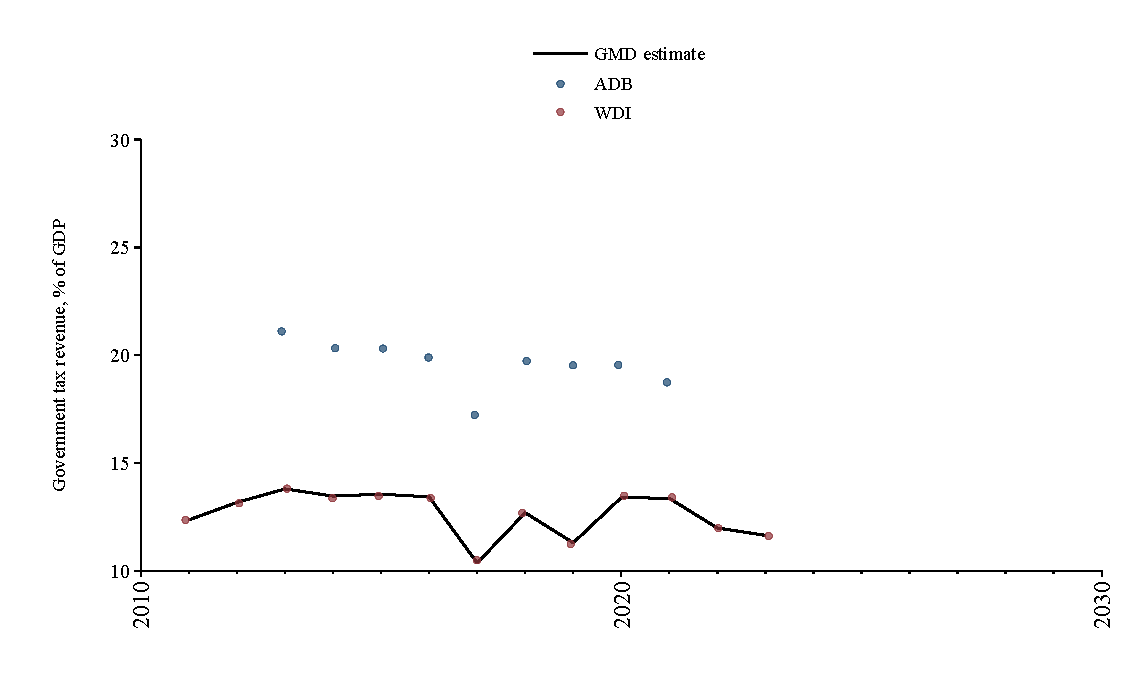
\includegraphics[width=\textwidth,height=0.6\textheight,keepaspectratio]{graphs/UZB_govtax_GDP.pdf}
\end{figure}
\end{minipage}
\end{adjustbox}
\begin{adjustbox}{max totalsize={\paperwidth}{\paperheight},center}
\begin{minipage}[t][\textheight][t]{\textwidth}
\vspace*{0.5cm}
\phantomsection
\addcontentsline{toc}{section}{Imports}
\begin{center}
{\Large\bfseries Imports}
\end{center}
\vspace{0.5cm}
\begin{table}[H]
\centering
\small
\begin{tabular}{|l|l|l|}
\hline
\textbf{Source} & \textbf{Time span} & \textbf{Notes} \\
\hline
\rowcolor{white}\cite{UN}& 1990 - 1996 &Spliced using overlapping data in 1997: (ratio = 104.6\%). \\
\rowcolor{lightgray}\cite{WDI}& 1997 - 2023 &Baseline source, overlaps with base year 2018. \\
\rowcolor{white}\cite{IMF_WEO_forecast}& 2024 - 2029 &Spliced using overlapping data in 2030. \\
\hline
\end{tabular}
\end{table}
\begin{figure}[H]
\centering
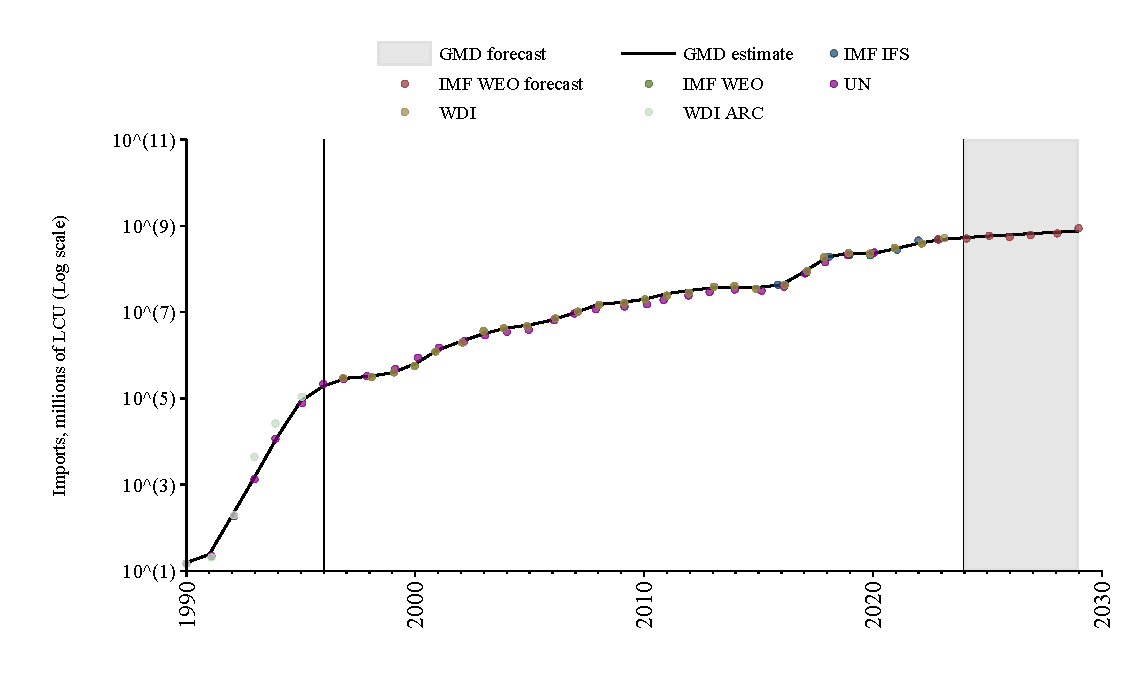
\includegraphics[width=\textwidth,height=0.6\textheight,keepaspectratio]{graphs/UZB_imports.pdf}
\end{figure}
\end{minipage}
\end{adjustbox}
\begin{adjustbox}{max totalsize={\paperwidth}{\paperheight},center}
\begin{minipage}[t][\textheight][t]{\textwidth}
\vspace*{0.5cm}
\phantomsection
\addcontentsline{toc}{section}{Imports to GDP ratio}
\begin{center}
{\Large\bfseries Imports to GDP ratio}
\end{center}
\vspace{0.5cm}
\begin{table}[H]
\centering
\small
\begin{tabular}{|l|l|l|}
\hline
\textbf{Source} & \textbf{Time span} & \textbf{Notes} \\
\hline
\rowcolor{white}\cite{UN}& 1990 - 1996 &Spliced using overlapping data in 1997: (ratio = 125.6\%). \\
\rowcolor{lightgray}\cite{WDI}& 1997 - 2023 &Baseline source, overlaps with base year 2018. \\
\rowcolor{white}\cite{IMF_WEO_forecast}& 2024 - 2029 &Spliced using overlapping data in 2030. \\
\hline
\end{tabular}
\end{table}
\begin{figure}[H]
\centering
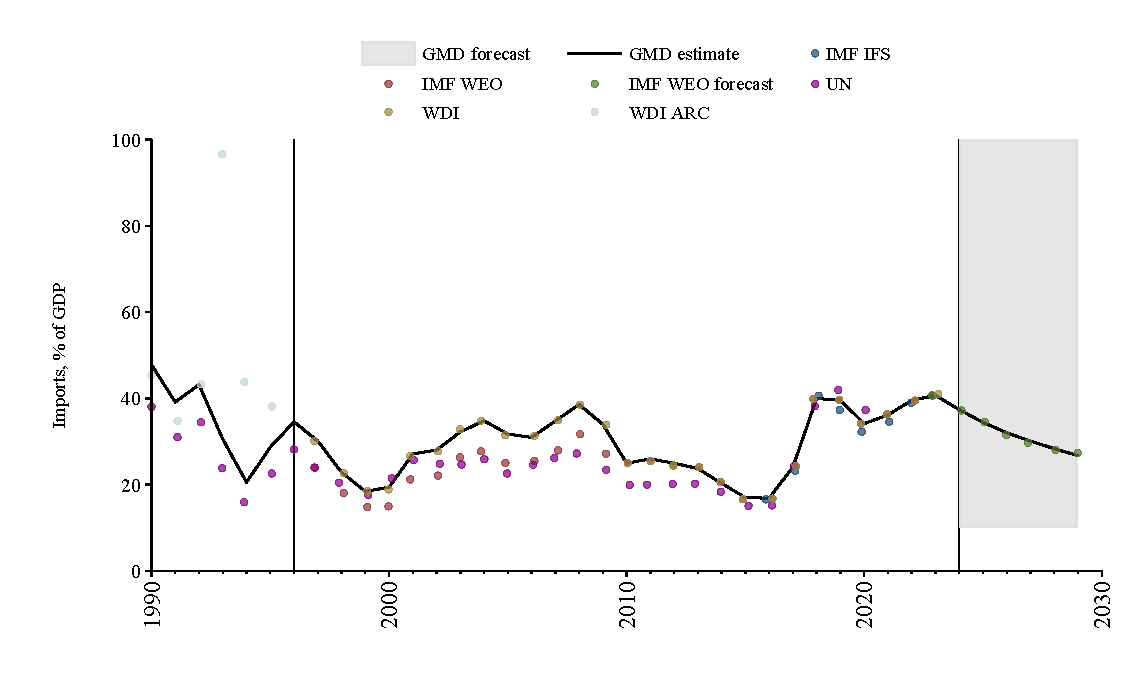
\includegraphics[width=\textwidth,height=0.6\textheight,keepaspectratio]{graphs/UZB_imports_GDP.pdf}
\end{figure}
\end{minipage}
\end{adjustbox}
\begin{adjustbox}{max totalsize={\paperwidth}{\paperheight},center}
\begin{minipage}[t][\textheight][t]{\textwidth}
\vspace*{0.5cm}
\phantomsection
\addcontentsline{toc}{section}{Inflation}
\begin{center}
{\Large\bfseries Inflation}
\end{center}
\vspace{0.5cm}
\begin{table}[H]
\centering
\small
\begin{tabular}{|l|l|l|}
\hline
\textbf{Source} & \textbf{Time span} & \textbf{Notes} \\
\hline
\rowcolor{white}\cite{WB_CC}& 1992 - 2023 &Baseline source, overlaps with base year 2018. \\
\rowcolor{lightgray}\cite{WDI}& 2024 - 2024 &Spliced using overlapping data in 2025. \\
\rowcolor{white}\cite{IMF_WEO_forecast}& 2025 - 2029 &Spliced using overlapping data in 2030. \\
\hline
\end{tabular}
\end{table}
\begin{figure}[H]
\centering
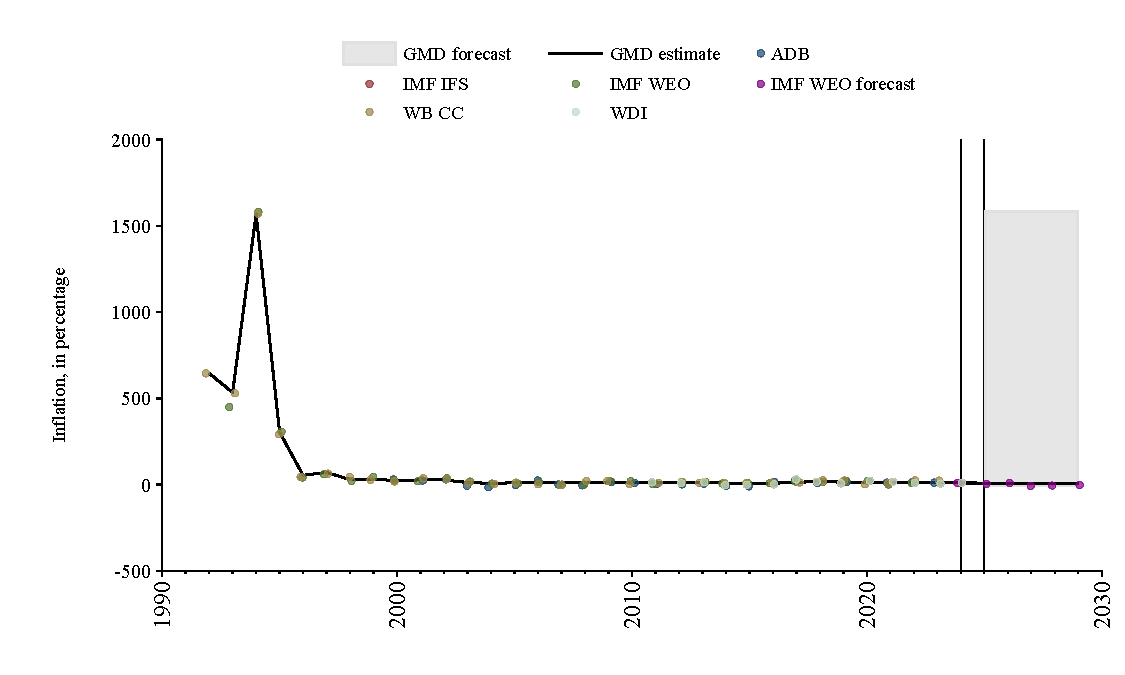
\includegraphics[width=\textwidth,height=0.6\textheight,keepaspectratio]{graphs/UZB_infl.pdf}
\end{figure}
\end{minipage}
\end{adjustbox}
\begin{adjustbox}{max totalsize={\paperwidth}{\paperheight},center}
\begin{minipage}[t][\textheight][t]{\textwidth}
\vspace*{0.5cm}
\phantomsection
\addcontentsline{toc}{section}{Investment}
\begin{center}
{\Large\bfseries Investment}
\end{center}
\vspace{0.5cm}
\begin{table}[H]
\centering
\small
\begin{tabular}{|l|l|l|}
\hline
\textbf{Source} & \textbf{Time span} & \textbf{Notes} \\
\hline
\rowcolor{white}\cite{WDI_ARC}& 1987 - 1989 &Spliced using overlapping data in 1990: (ratio = 100.4\%). \\
\rowcolor{lightgray}\cite{UN}& 1990 - 1991 &Spliced using overlapping data in 1992: (ratio = 79.8\%). \\
\rowcolor{white}\cite{WDI}& 1992 - 2023 &Baseline source, overlaps with base year 2018. \\
\rowcolor{lightgray}\cite{IMF_WEO_forecast}& 2024 - 2029 &Spliced using overlapping data in 2030. \\
\hline
\end{tabular}
\end{table}
\begin{figure}[H]
\centering
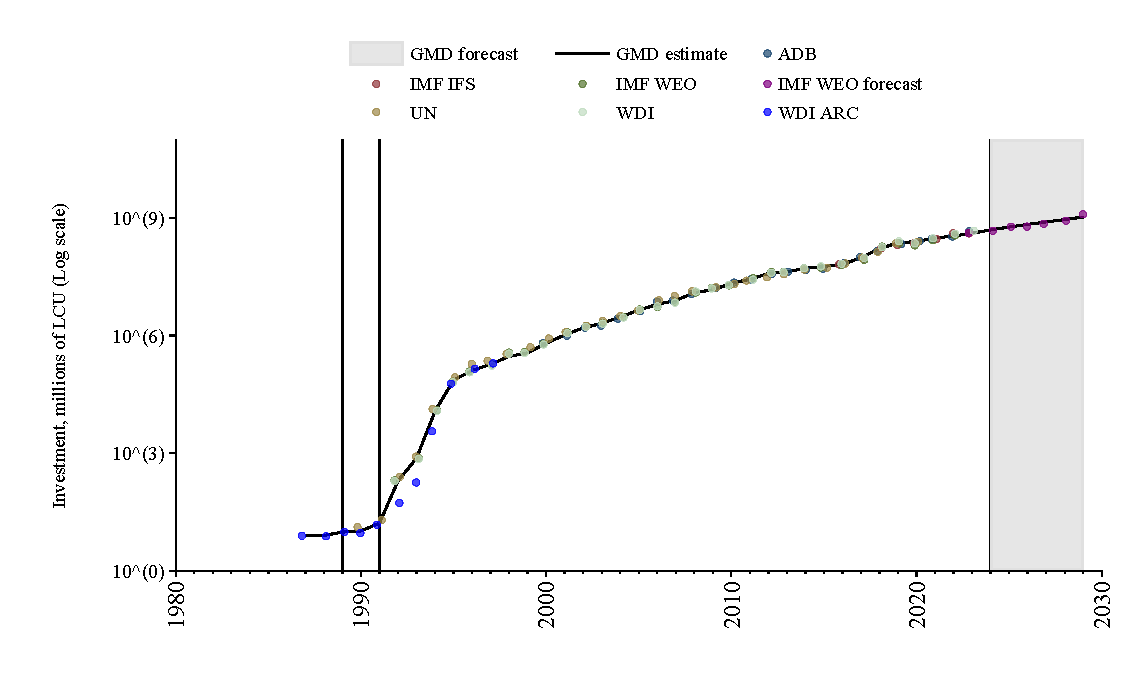
\includegraphics[width=\textwidth,height=0.6\textheight,keepaspectratio]{graphs/UZB_inv.pdf}
\end{figure}
\end{minipage}
\end{adjustbox}
\begin{adjustbox}{max totalsize={\paperwidth}{\paperheight},center}
\begin{minipage}[t][\textheight][t]{\textwidth}
\vspace*{0.5cm}
\phantomsection
\addcontentsline{toc}{section}{Investment to GDP ratio}
\begin{center}
{\Large\bfseries Investment to GDP ratio}
\end{center}
\vspace{0.5cm}
\begin{table}[H]
\centering
\small
\begin{tabular}{|l|l|l|}
\hline
\textbf{Source} & \textbf{Time span} & \textbf{Notes} \\
\hline
\rowcolor{white}\cite{WDI_ARC}& 1987 - 1991 &Spliced using overlapping data in 1992: (ratio = 335.1\%). \\
\rowcolor{lightgray}\cite{WDI}& 1992 - 2023 &Baseline source, overlaps with base year 2018. \\
\rowcolor{white}\cite{IMF_WEO_forecast}& 2024 - 2029 &Spliced using overlapping data in 2030. \\
\hline
\end{tabular}
\end{table}
\begin{figure}[H]
\centering
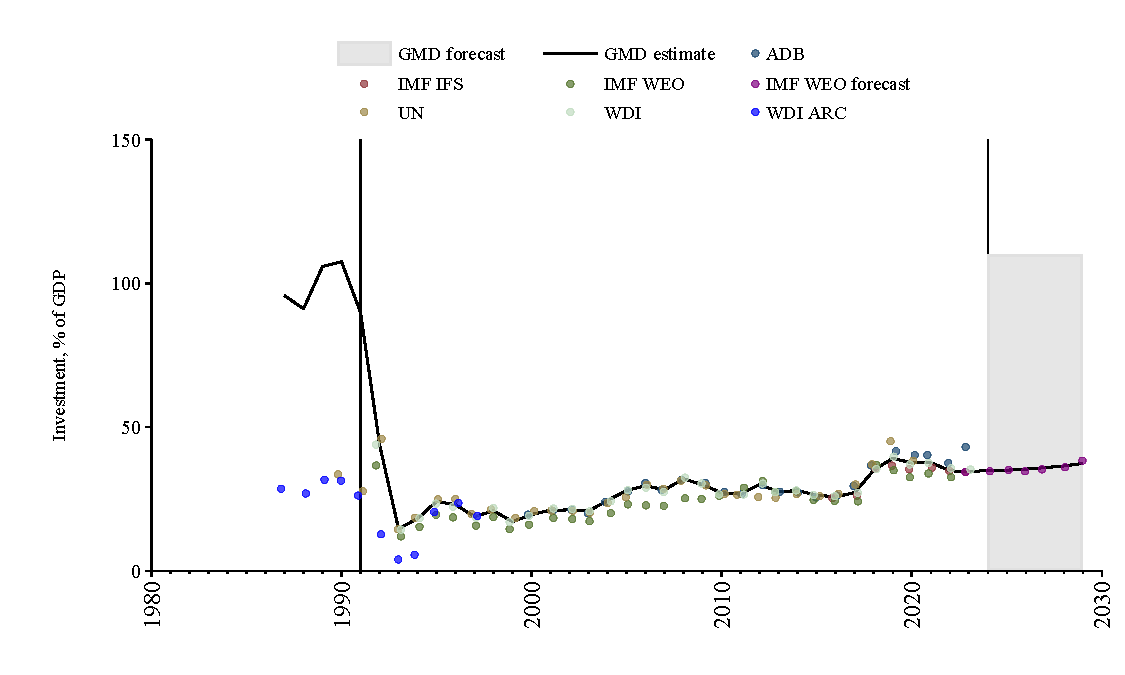
\includegraphics[width=\textwidth,height=0.6\textheight,keepaspectratio]{graphs/UZB_inv_GDP.pdf}
\end{figure}
\end{minipage}
\end{adjustbox}
\begin{adjustbox}{max totalsize={\paperwidth}{\paperheight},center}
\begin{minipage}[t][\textheight][t]{\textwidth}
\vspace*{0.5cm}
\phantomsection
\addcontentsline{toc}{section}{Nominal GDP}
\begin{center}
{\Large\bfseries Nominal GDP}
\end{center}
\vspace{0.5cm}
\begin{table}[H]
\centering
\small
\begin{tabular}{|l|l|l|}
\hline
\textbf{Source} & \textbf{Time span} & \textbf{Notes} \\
\hline
\rowcolor{white}\cite{WDI}& 1987 - 2023 &Baseline source, overlaps with base year 2018. \\
\rowcolor{lightgray}\cite{IMF_WEO_forecast}& 2024 - 2029 &Spliced using overlapping data in 2030. \\
\hline
\end{tabular}
\end{table}
\begin{figure}[H]
\centering
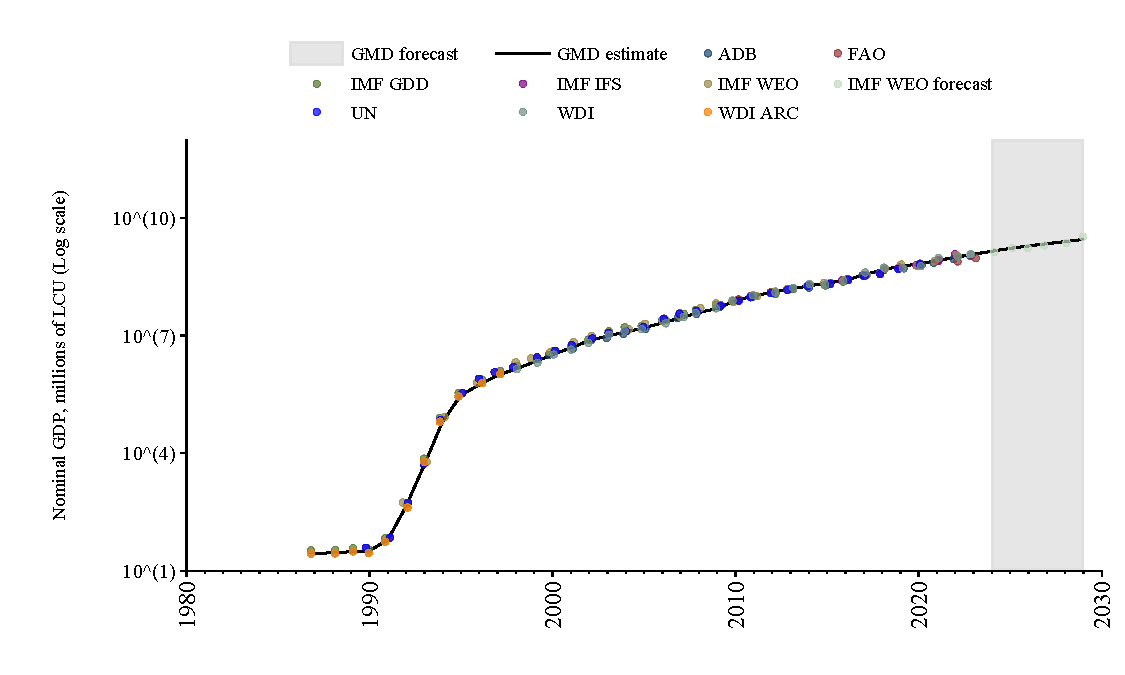
\includegraphics[width=\textwidth,height=0.6\textheight,keepaspectratio]{graphs/UZB_nGDP.pdf}
\end{figure}
\end{minipage}
\end{adjustbox}
\begin{adjustbox}{max totalsize={\paperwidth}{\paperheight},center}
\begin{minipage}[t][\textheight][t]{\textwidth}
\vspace*{0.5cm}
\phantomsection
\addcontentsline{toc}{section}{Population}
\begin{center}
{\Large\bfseries Population}
\end{center}
\vspace{0.5cm}
\begin{table}[H]
\centering
\small
\begin{tabular}{|l|l|l|}
\hline
\textbf{Source} & \textbf{Time span} & \textbf{Notes} \\
\hline
\rowcolor{white}\cite{Gapminder}& 1800 - 1949 &Spliced using overlapping data in 1950: (ratio = 96.7\%). \\
\rowcolor{lightgray}\cite{IMF_IFS}& 1950 - 1959 &Spliced using overlapping data in 1960: (ratio = 96.3\%). \\
\rowcolor{white}\cite{WDI}& 1960 - 2023 &Baseline source, overlaps with base year 2018. \\
\rowcolor{lightgray}\cite{Gapminder}& 2024 - 2030 &Spliced using overlapping data in 2031: (ratio = 99.9\%). \\
\hline
\end{tabular}
\end{table}
\begin{figure}[H]
\centering
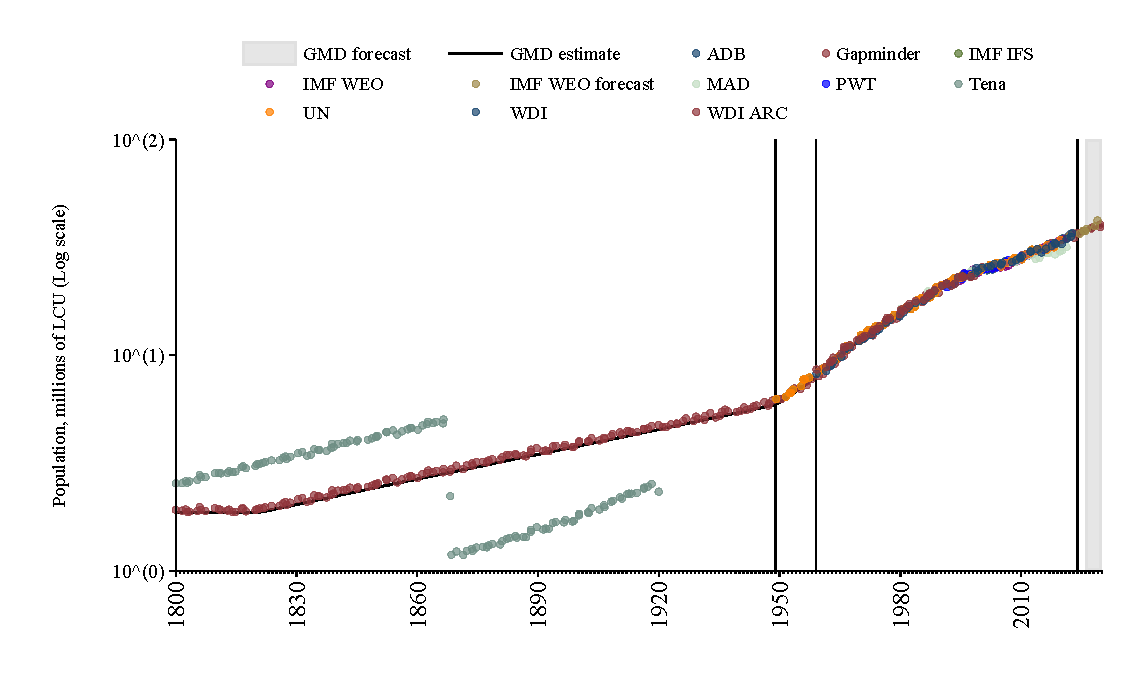
\includegraphics[width=\textwidth,height=0.6\textheight,keepaspectratio]{graphs/UZB_pop.pdf}
\end{figure}
\end{minipage}
\end{adjustbox}
\begin{adjustbox}{max totalsize={\paperwidth}{\paperheight},center}
\begin{minipage}[t][\textheight][t]{\textwidth}
\vspace*{0.5cm}
\phantomsection
\addcontentsline{toc}{section}{Real GDP}
\begin{center}
{\Large\bfseries Real GDP}
\end{center}
\vspace{0.5cm}
\begin{table}[H]
\centering
\small
\begin{tabular}{|l|l|l|}
\hline
\textbf{Source} & \textbf{Time span} & \textbf{Notes} \\
\hline
\rowcolor{white}\cite{WDI_ARC}& 1979 - 1979 &Spliced using overlapping data in 1980. \\
\rowcolor{lightgray}\cite{MAD}& 1980 - 1986 &Spliced using overlapping data in 1987. \\
\rowcolor{white}\cite{WDI}& 1987 - 2023 &Baseline source, overlaps with base year 2018. \\
\rowcolor{lightgray}\cite{IMF_WEO_forecast}& 2024 - 2029 &Spliced using overlapping data in 2030. \\
\hline
\end{tabular}
\end{table}
\begin{figure}[H]
\centering
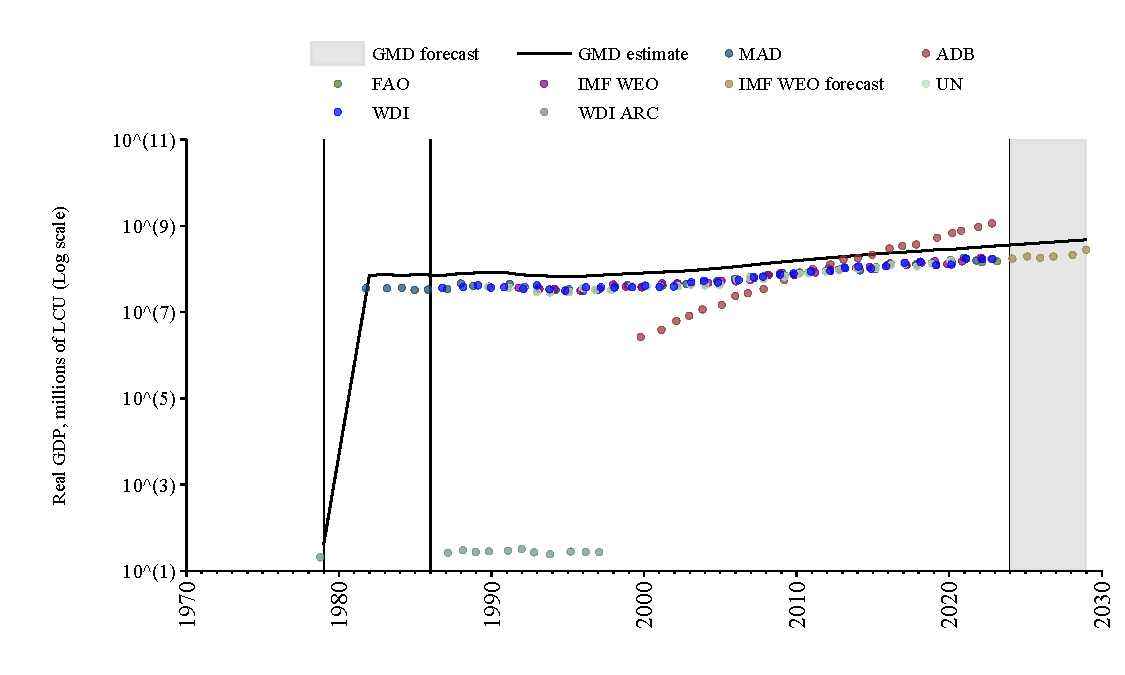
\includegraphics[width=\textwidth,height=0.6\textheight,keepaspectratio]{graphs/UZB_rGDP.pdf}
\end{figure}
\end{minipage}
\end{adjustbox}
\begin{adjustbox}{max totalsize={\paperwidth}{\paperheight},center}
\begin{minipage}[t][\textheight][t]{\textwidth}
\vspace*{0.5cm}
\phantomsection
\addcontentsline{toc}{section}{Real total consumption}
\begin{center}
{\Large\bfseries Real total consumption}
\end{center}
\vspace{0.5cm}
\begin{table}[H]
\centering
\small
\begin{tabular}{|l|l|l|}
\hline
\textbf{Source} & \textbf{Time span} & \textbf{Notes} \\
\hline
\rowcolor{white}\cite{UN}& 1990 - 1994 &Spliced using overlapping data in 1995. \\
\rowcolor{lightgray}\cite{WDI}& 1995 - 2023 &Baseline source, overlaps with base year 2018. \\
\hline
\end{tabular}
\end{table}
\begin{figure}[H]
\centering
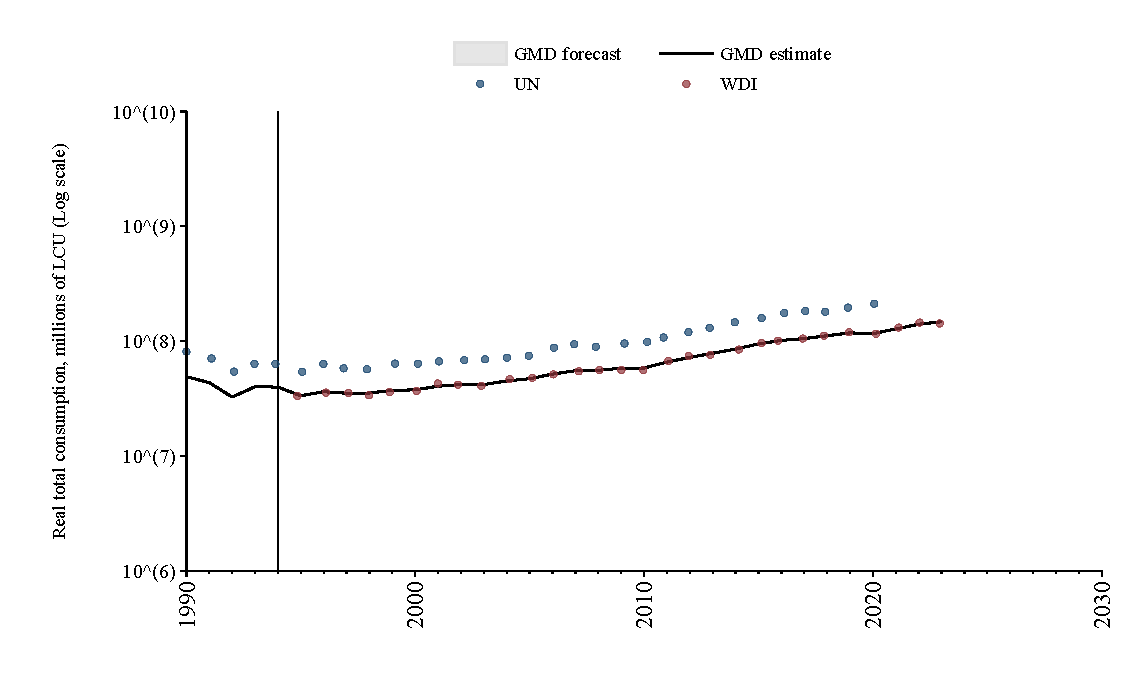
\includegraphics[width=\textwidth,height=0.6\textheight,keepaspectratio]{graphs/UZB_rcons.pdf}
\end{figure}
\end{minipage}
\end{adjustbox}
\begin{adjustbox}{max totalsize={\paperwidth}{\paperheight},center}
\begin{minipage}[t][\textheight][t]{\textwidth}
\vspace*{0.5cm}
\phantomsection
\addcontentsline{toc}{section}{Short term interest rate}
\begin{center}
{\Large\bfseries Short term interest rate}
\end{center}
\vspace{0.5cm}
\begin{table}[H]
\centering
\small
\begin{tabular}{|l|l|l|}
\hline
\textbf{Source} & \textbf{Time span} & \textbf{Notes} \\
\hline
\rowcolor{white}\cite{IMF_IFS}& 2018 - 2024 &Baseline source, overlaps with base year 2018. \\
\hline
\end{tabular}
\end{table}
\begin{figure}[H]
\centering
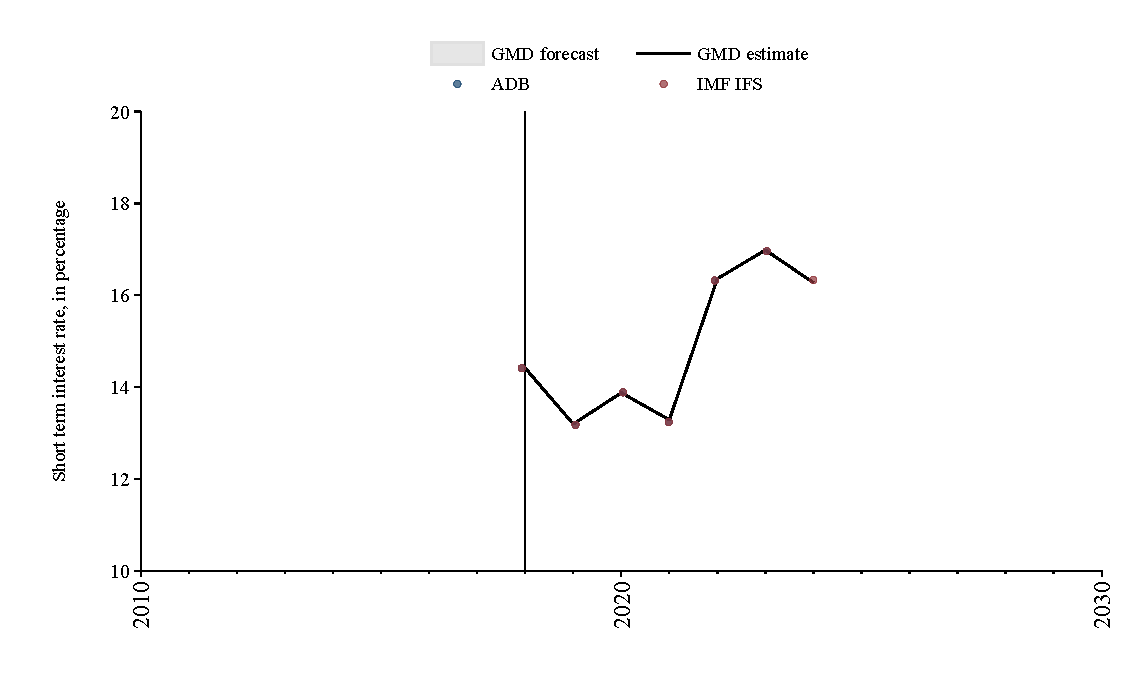
\includegraphics[width=\textwidth,height=0.6\textheight,keepaspectratio]{graphs/UZB_strate.pdf}
\end{figure}
\end{minipage}
\end{adjustbox}
\begin{adjustbox}{max totalsize={\paperwidth}{\paperheight},center}
\begin{minipage}[t][\textheight][t]{\textwidth}
\vspace*{0.5cm}
\phantomsection
\addcontentsline{toc}{section}{Unemployment}
\begin{center}
{\Large\bfseries Unemployment}
\end{center}
\vspace{0.5cm}
\begin{table}[H]
\centering
\small
\begin{tabular}{|l|l|l|}
\hline
\textbf{Source} & \textbf{Time span} & \textbf{Notes} \\
\hline
\rowcolor{white}\cite{ADB}& 2000 - 2023 &Baseline source, overlaps with base year 2018. \\
\rowcolor{lightgray}\cite{IMF_WEO_forecast}& 2024 - 2029 &Spliced using overlapping data in 2030. \\
\hline
\end{tabular}
\end{table}
\begin{figure}[H]
\centering
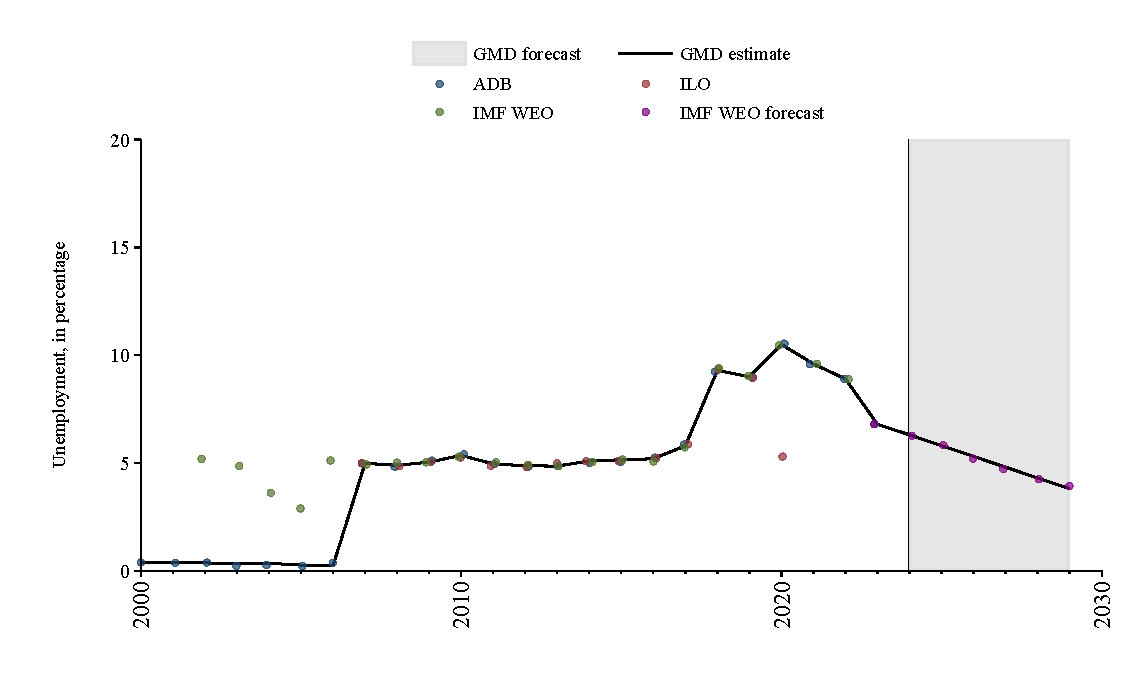
\includegraphics[width=\textwidth,height=0.6\textheight,keepaspectratio]{graphs/UZB_unemp.pdf}
\end{figure}
\end{minipage}
\end{adjustbox}
\phantomsection
\addcontentsline{toc}{section}{References}
\begin{center}
{\Large\bfseries References}
\end{center}
\small
\bibliographystyle{qje}
\bibliography{bib}
\end{document}
